\documentclass[a4paper, 11pt, normalem]{report}

\usepackage{../../../LaTeX-Templates/Notes}

\usetikzlibrary{decorations.pathmorphing}
\usetikzlibrary{arrows.meta}

\tikzset{snake it/.style={decorate,decoration=snake}}

\title{Intro to \\ Soft Condensed Matter \vspace{-20pt}}
\author{Dr Voitchovsky}
\date{\vspace{-15pt}Epiphany Term 2019}
\rhead{\hyperlink{page.1}{Contents}}

\begin{document}
\maketitle
\tableofcontents

\chapter{General Introduction to Soft Condensed Matter}
\section{Outline}
\begin{itemize}
    \item General introduction to Soft Condensed Matter - main characteristics
    \item Intermolecular forces
        \begin{itemize}
            \item solid
            \item liquid
            \item gas
        \end{itemize}
\end{itemize}

\section{What is Soft Matter?}
Some typical examples:
\begin{itemize}
    \item Polymers (chain of molecules), i.e. plastics, woods, DNA
    \item Colloids (solid particles suspended in a liquid), i.e. milk, paint
    \item Foams, emulsion (liquid/gas droplets in a liquid), i.e. mayo, dressing
    \item Liquid crystals (liquid formed of particles that can be oriented), i.e displays, optics
    \item Supramolecular selfassemblies (ordered hierarchical structures holding together without covalent bonds) i.e. humans
\end{itemize}

The term 'Soft Matter' intuitively suggests the ability for matter to deform or reshape easily when subjected to 'moderate' external constraints (e.g. liquids, gels, rubber,...).
In practice, formalising this intuitive definition has several implications:
\begin{itemize}
    \item structural organisation and symmetry of the material
    \item scale (spatial and temporal) of the observation
\end{itemize}
Let's take some examples: {\color{blue}water} + {\color{red}gelatin} $\to$ {\color{green}mix}
\begin{table}[H]
    \centering
    \begin{tabular}{c|l|l}
        & molecular level & macroscopic level \\
        \hline
        \multirow{3}{*}{structure} & {\color{blue} network of H-bonds} & {\color{blue}liquid} \\
                                   & {\color{red} molcular chains} & {\color{red} solid} \\
                                   & {\color{green} wter-filled mesh} & {\color{green} gel} \\
        \hline
        \multirow{3}{*}{timescale} & {\color{blue} ps} & {\color{blue} ms} \\
                                   & {\color{red} min - day} & {\color{red} year (elastic)} \\
                                   & {\color{green} ns - ms} & {\color{green} depends}
    \end{tabular}
\end{table}
Soft materials are very often a mixture of solids, liquids, and/or gases structured at the mesoscopic scale.
\begin{table}[H]
    \centering
    \begin{tabular}{c|p{2.5cm}|p{2.5cm}|p{2.5cm}}
        & Solid & Liquid & Gas \\
        \hline
        Solid & polymers, $\mu$m & colloids, nm $\to$ \newline gels, $\mu$m & foam \\
        \hline
        Liquid & & mixtures, nm  \newline emulsions, $\mu$m & emulsions \newline foams \\
        \hline
        Gas & & & {\large X}
    \end{tabular}
\end{table}

\section{Some key themes of Soft Matter}
\begin{itemize}
    \item Scale: nm $\to$ $\mu$m (ns $\to$ ms)
    \item Soft matter usually exhibits some mesoscopic substructure on the nanameter to micrometer scale - universality.
    \item Atomic details are most of the time not important or required to describe the behaviour of soft matter.
    The relevant details are that of the mesescopic structure.
    \item Thermal fluctuations, $k_BT \approx 4\times10^{-21}\,J \approx 0.03\,eV$ - the energy to assemble/disassemble, or distort arrangement of substructure is typically in the order of $k_BT$.
    \item Many soft matter systems are formed by spontaneous self-assembly of molecules occurring under certain conditions.
    \item As for any condensed matter, most of the macroscopic properties and characteristics of Soft Matter is governed by the interaction potential between molecules.
\end{itemize}

\section{Intermolecular forces}
In order for condensed matter to exist (solid, liquid), there must be an attractive force larger than thermal fluctuations that operate between separated molecules.
At short range, a repulsive force allows molecules not to collapse into one another.
Stability:
\begin{align}
    |\e| &> k_BT \\
    F &= -\frac{\p}{\p r} U(r)
\end{align}
\vspace{-20pt}
\begin{figure}[H]
    \centering
    \begin{tikzpicture}
        \draw[thick,->] (0,0) -- (6,0) node[anchor=north west] {r};
        \draw[thick,->] (0,-2) -- (0,2) node[anchor=south east] {U(r)};
        \draw (0.2,2) .. controls (2,-5) and (4,0) .. (5.8,-0.2);
        \draw[red,thick,dashed] (2.5,0) node[black,anchor=south] {$r_l$} -- (2.5,-1.8);
        \draw[red,thick,dashed] (0,-1.8) node[black,anchor=east] {$\e_l < 0$} -- (2.5,-1.8);
        \draw[black,decorate,decoration={brace,amplitude=10pt,mirror},yshift=-2pt] (0,-1.8) -- (2.5,-1.8) node[black,midway,anchor=north,yshift=-8pt] {repulsive};
        \draw[black,decorate,decoration={brace,amplitude=10pt,mirror},yshift=-2pt] (2.5,-1.8) -- (6,-1.8) node[black,midway,anchor=north,yshift=-8pt] {attractive};
    \end{tikzpicture}
\end{figure}
\vspace{-80pt}
Fundamentally, all intermolecular forces are of electrostatic origin (i.e. not nuclear or gravitational).
It is helpful to categorise them as follows:
\textbf{Repulsive forces:}
\begin{itemize}
    \item Characteristic - strong, short range, stop matter from collapsing
    \item Mechanism - Pauli repulsion between $e^-$ orbitals of neighbouring molecules
\end{itemize}
\textbf{Attractive forces:}
\begin{itemize}
      \item Characteristic - weaker and longer range than repulsive forces
      \item Mechanism - several mechanisms (and hence forces) can be distinguished; they are classified hereafter by order of strength:
        \begin{itemize}
            \item Hydrophobic interactions: Driven by hydrogen-bonding solvents in order to minimise contact with non-hydrogen bonding molecules (hydrophobic molecules).
                $\e \approx 2-5\,k_BT$, indirect, proportional to area.
            \item Hydrogen bonds: Form between electropositive hydrogen atom and electronegative oxygen.
                $\e \approx 1.5-15\,k_BT$.
            \item Ionic interactions: Occur between particles with opposite charges, $q_1$ and $q_2$, and is relatively long range and can easily be screened by other charged or polar molecules.
                $\e \approx 50-300\,k_BT$.
                \begin{equation}
                    U(r) = \frac{q_1q_2}{4\pi\e\e_0 r^2}
                \end{equation}
            \item Covalent bonds: Due to electrons of contributing atoms interacting with more than 1 atom to reduce the system energy, hence creating stable molecular orbitals.
                $\e \approx 100-400\,k_BT$.
        \end{itemize}
\end{itemize}

\section{Solid Vs Liquid Vs Gas (At Equilibrium)}
It is possible to qualitatively understand the different phases of a material (at equilibrium) simply in terms of the magnitude of the pair interaction potential $U_{attract}$.
\begin{table}[H]
    \centering
    \begin{tabular}{l|l|l}
        Solid & Liquid & Gas \\
        \hline
        $U_{attract} > k_BT$ & $U_{attract} \approx k_BT$ & $U_{attract} << k_BT$ \\
        stays in place & stays together after collision & occasional collisions \\
        long range order & correlation (local) & no correlation \\
        ordered packing & random & no packing
    \end{tabular}
\end{table}
The equilibrium between different phases is usually described by phase diagrams, for example with pressure (P) vs temperature (T).
\begin{figure}[H]
    \centering
    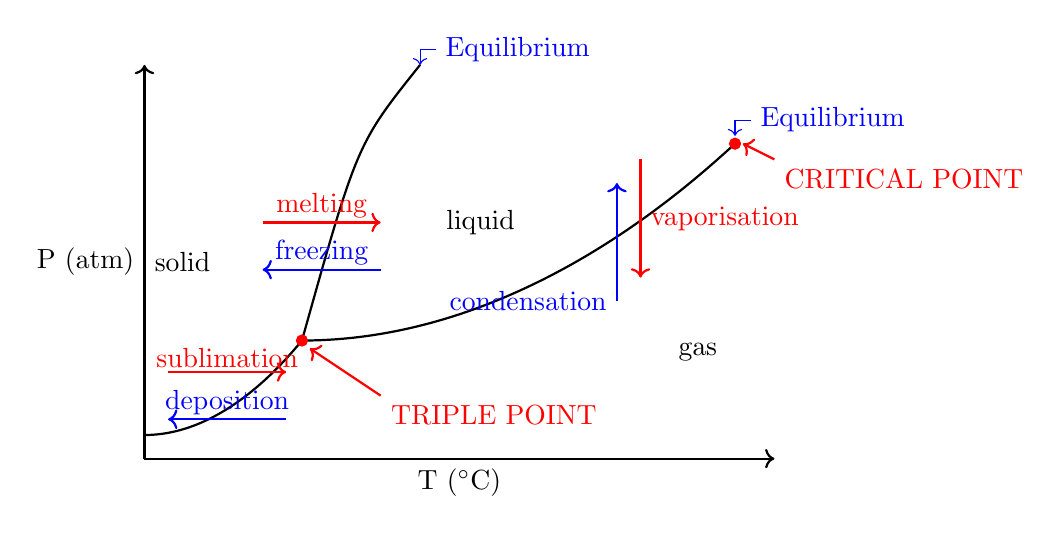
\begin{tikzpicture}
        \draw[thick,->] (0,0) -- (8,0) node[midway,anchor=north] {T ($^\circ$C)};
        \draw[thick,->] (0,0) -- (0,5) node[midway,anchor=east] {P (atm)} node[midway,anchor=west] {solid};
        \draw[thick] (0,0.3) parabola (2,1.5);
        \draw[thick] (2,1.5) .. controls (2.7,4) .. (3.5,5);
        \draw[thick] (2,1.5) parabola (7.5,4);
        \draw[->,blue] (3.7,5.2) node[anchor=west] {Equilibrium} -- (3.5,5.2) -- (3.5,5);
        \draw[->,blue] (7.7,4.3) node[anchor=west] {Equilibrium} -- (7.5,4.3) -- (7.5,4.1);
        \draw[->,red,thick] (1.5,3) -- (3,3) node[midway,anchor=south,yshift=-2pt] {melting} node[anchor=west,xshift=20pt,black] {liquid};
        \draw[->,blue,thick] (3,2.4) -- (1.5,2.4) node[midway,anchor=south,yshift=-2pt] {freezing};
        \draw[->,red,thick] (0.3,1.1) -- (1.8,1.1) node[midway,anchor=south,yshift=-2pt] {sublimation};
        \draw[->,blue,thick] (1.8,0.5) -- (0.3,0.5) node[midway,anchor=south,yshift=-2pt] {deposition};
        \filldraw[red] (2,1.5) circle (2pt);
        \filldraw[red] (7.5,4) circle (2pt);
        \draw[->,thick,red] (3,0.8) node[anchor=north west] {TRIPLE POINT} -- (2.1,1.4);
        \draw[->,thick,blue] (6,2) node[anchor=east] {condensation} -- (6,3.5);
        \draw[->,thick,red] (6.3,3.8) -- (6.3,2.3) node[midway,anchor=west] {vaporisation} node[black,anchor=north west,xshift=10pt,yshift=-20pt] {gas};
        \draw[->,thick,red] (8,3.8) node[anchor=north west] {CRITICAL POINT} -- (7.6,4);
    \end{tikzpicture}
\end{figure}

\chapter{Relevant timescale and physical properties}
\section{Outline}
\begin{itemize}
    \item Response of soft condensed matter to mechanical stress
    \item Macroscopic level
        \begin{equation*}
            \text{viscoelastic } \begin{cases} \text{ solid (elastic)} \\ \text{ liquid (viscous)}\end{cases}
        \end{equation*}
    \item Molecular picture
    \item Glass
\end{itemize}

Key concepts of CMP:
\begin{itemize}
    \item Timescale
    \item Relevant spatial scale
    \item thermal fluctuations
    \item intermolecular potentials
\end{itemize}

\section{Response of condensed matter to shear stress}
Condensed matter is usually in one of two states: solid or liquid.
Soft matter can simulataneously have attributes of both in its response to an applied stress.
Let's start by examining the behaviour of ideal solids and liquids subjected to shear stress.

\subsection{Hookean solids}
A solid that has a perfectly elastic behaviour is called \emph{Hookean.}
Practically, this is true only for perfect solids (single crystals) but it is a reasonable approximation for most 'hard' solids under a small, non-destructive stress.
\begin{itemize}
    \item Applying a shear stress, $\sigma$, to a Hookean solid results in a proportional shear strain, $e$
    \item The shear stress is proportional to the shear strain and the proportionality constant is the shear modulus $G$.
\end{itemize}
\begin{figure}[H]
    \centering
    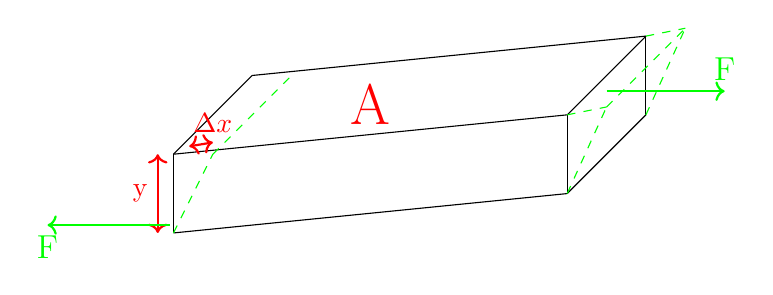
\begin{tikzpicture}
        \draw (0,0) -- (5,0.5);
        \draw (5,0.5) -- (6,1.5);
        \draw (6,1.5) -- (6,2.5);
        \draw (5,0.5) -- (5,1.5);
        \draw (0,1) -- (5,1.5) node[anchor=south,red,midway] {\huge A};
        \draw (0,1) -- (1,2);
        \draw (0,0) -- (0,1);
        \draw[thick,red,<->] (-0.2,0) -- (-0.2,1) node[anchor=east,midway] {y};
        \draw (5,1.5) -- (6,2.5);
        \draw (1,2) -- (6,2.5);
        \draw[thick,green,->] (5.5,1.8) -- (7,1.8) node[anchor=south] {\large F};
        \draw[thick,green,->] (-0.05,0.1) -- (-1.6,0.1) node[anchor=north] {\large F};
        \draw[green,dashed] (0.5,1) -- (1.5,2);
        \draw[thick,red,<->] (0.2,1.1) -- (0.5,1.15) node[anchor=south] {$\Delta x$};
        \draw[green,dashed] (0,0) -- (0.5,1);
        \draw[green,dashed] (5,0.5) -- (5.5,1.6);
        \draw[green,dashed] (6,1.5) -- (6.5,2.6);
        \draw[green,dashed] (5.5,1.6) -- (6.5,2.6);
        \draw[green,dashed] (5,1.5) -- (5.5,1.6);
        \draw[green,dashed] (6,2.5) -- (6.5,2.6);
    \end{tikzpicture}
\end{figure}
\begin{align}
    \sigma &= \frac{F}{A}, \text{ stress, } \left[\frac{N}{m^2}\right] \\
    e &= \frac{\Delta x}{y}, \text{ strain} \\
    \sigma &= Ge,~ G - \text{ shear modulus, } \left[\frac{N}{m^2}\right]
\end{align}

\subsection{Newtonian Liquids}
A Newtonian liquid is chartered by a single, time- and shear rate- independent, viscosity.
Water is a typical example of a Newtonian liquid.
\begin{itemize}
    \item An applied shear stress, $\sigma$, produces a flow with a constant shear strain \unl{rate}, $\dot{e}$, in response.
    \item The shear stress strain is proportional to the shear rate and the proportionality constant is the viscosity, $\eta$.
\end{itemize}
\begin{align}
    \sigma &= \frac FA \\
    \dot{e} &= \frac{\Delta\dot{x}}{y} \\
    \sigma &= \eta\dot{e},~ \eta - \text{ viscosity, } \left[\frac{Ns}{m^2}\right]
\end{align}
In reality, many materials - particularly soft matter - tend to behave in a way that combines viscous and elastic response, depending on the timescale considered.
This is known as \textbf{viscoelasticity.}\\
Imagine we apply a sudden constant shear stress to a material and examine the evolution of the induced strain with time:
\begin{multicols}{2}
    \begin{center}
    \textbf{Ideal (Hookean) Solid:}
    \begin{figure}[H]
        \centering
        \begin{tikzpicture}
            \draw[thick,->] (0,0) node[anchor=north east] {0} -- (0,4) node[anchor=south east] {e};
            \draw[thick,->] (0,0) -- (4,0) node[anchor=north west] {t};
            \draw (0,2) node[anchor=east] {\Large $\frac{\sigma}{G}$} -- (3.8,2);
        \end{tikzpicture}
    \end{figure}
    \end{center}
    \columnbreak
    \begin{center}
    \textbf{Ideal (Newtonian) Liquid:}
    \begin{figure}[H]
        \centering
        \begin{tikzpicture}
            \draw[thick,->] (0,0) node[anchor=north east] {0} -- (0,4) node[anchor=south east] {e};
            \draw[thick,->] (0,0) -- (4,0) node[anchor=north west] {t};
            \draw (0,0) -- (3.5,3.5);
            \draw (1.2,1.2) -- (2.2,1.2);
            \draw (2.2,1.2) -- (2.2,2.2) node[anchor=west,midway] {\Large $\dot{e} = \frac{\sigma}{\eta}$};
        \end{tikzpicture}
    \end{figure}
    \end{center}
\end{multicols}
\begin{figure}[H]
    \centering
    \begin{tikzpicture}
        \draw[thick,->] (0,0) node[anchor=north east] {0} -- (0,6) node[anchor=south east] {e};
        \draw[thick,->] (0,0) -- (8,0) node[anchor=north west] {t} node[anchor=south,yshift=35pt] {\Large $\tau \approx \frac{\eta}{G_0}$};
        \draw (0,3) node[anchor=east] {\Large $\frac{\sigma}{G_0}$} -- (4,3);
        \draw (4,3) -- (7.8,5.8);
        \draw[dashed] (0,0) -- (4,3);
        \draw[dashed] (4,0) node[anchor=north] {\Large $\tau$} -- (4,3);
        \draw (5,3.75) -- (7,3.75);
        \draw (7,3.75) -- (7,5.2) node[anchor=west,midway] {\Large $\frac{\sigma}{\eta}$};
    \end{tikzpicture}
\end{figure}
Practically, the viscoelastic response of most soft materials is often more complicated.
The relation $\eta \approx G_0\tau$ assumes a single relaxation timescale which may not be true, but it offers a framework for understanding the viscoelasticity at the molecular level.
At the macroscopic scale, the formalism of Newtonian liquids can be generalised to the viscoelastic behaviour of \emph{Complex Fluids} in a simple manner:
\begin{equation}
    \sigma = \eta(\dot{e})\,\dot{e}
\end{equation}
Three possible responses of a fluid to shear stress can be distinguished:
\begin{multicols}{3}
    \begin{center}
        \textbf{Newtonian:}
        \begin{figure}[H]
            \centering
            \begin{tikzpicture}
                \draw[thick,->] (0,0) -- (0,3) node[anchor=south east] {$\sigma$};
                \draw[thick,->] (0,0) -- (3,0) node[anchor=north west] {$\dot{e}$};
                \draw (0,0) -- (2.8,2.8);
                \draw (1.2,1.2) -- (1.8,1.2);
                \draw (1.8,1.2) -- (1.8,1.8) node[anchor=west,midway] {\Large $\eta$};
            \end{tikzpicture} \\
            \begin{tikzpicture}
                \draw[thick,->] (0,0) -- (0,3) node[anchor=south east] {$\eta_{\text{eff}}$};
                \draw[thick,->] (0,0) -- (3,0) node[anchor=north west] {$\dot{e}$};
                \draw (0,1.5) -- (2.8,1.5);
            \end{tikzpicture}
        \end{figure}
    \end{center}
    \columnbreak
    \begin{center}
        \textbf{Shear Thinning:}
        \begin{figure}[H]
            \centering
            \begin{tikzpicture}
                \draw[thick,->] (0,0) -- (0,3) node[anchor=south east] {$\sigma$};
                \draw[thick,->] (0,0) -- (3,0) node[anchor=north west] {$\dot{e}$};
                \draw (0,0) .. controls (1,2) .. (2.5,2.2);
            \end{tikzpicture} \\
            \begin{tikzpicture}
                \draw[thick,->] (0,0) -- (0,3) node[anchor=south east] {$\eta_{\text{eff}}$};
                \draw[thick,->] (0,0) -- (3,0) node[anchor=north west] {$\dot{e}$};
                \draw (0,2) .. controls (1.5,2) .. (2.5,0.5);
            \end{tikzpicture}
        \end{figure}
    \end{center}
    \columnbreak
    \begin{center}
        \textbf{Shear Thickening:}
        \begin{figure}[H]
            \centering
            \begin{tikzpicture}
                \draw[thick,->] (0,0) -- (0,3) node[anchor=south east] {$\sigma$};
                \draw[thick,->] (0,0) -- (3,0) node[anchor=north west] {$\dot{e}$};
                \draw (0,0) parabola (2.5,2.5);
            \end{tikzpicture} \\
            \begin{tikzpicture}
                \draw[thick,->] (0,0) -- (0,3) node[anchor=south east] {$\eta_{\text{eff}}$};
                \draw[thick,->] (0,0) -- (3,0) node[anchor=north west] {$\dot{e}$};
                \draw (0,1) parabola (2.5,2.5);
            \end{tikzpicture}
        \end{figure}
    \end{center}
\end{multicols}

\section{Response to (shear) stress at the molecular level}
The macroscopic response of matter to stress originates from displacement of atoms and molecules from their equilibrium position.
We can therefore relate the different moduli (shear, viscous, Young) to intermolecular forces and their respective evolution timescale.

\subsection{Solids}
\begin{multicols}{2}
    \begin{figure}[H]
        \centering
        \vspace{40pt}
        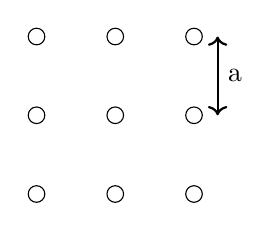
\begin{tikzpicture}
            \draw (0,0) circle (3pt);
            \draw (0,1) circle (3pt);
            \draw (0,2) circle (3pt);
            \draw (1,0) circle (3pt);
            \draw (1,1) circle (3pt);
            \draw (1,2) circle (3pt);
            \draw (2,0) circle (3pt);
            \draw (2,1) circle (3pt);
            \draw (2,2) circle (3pt);
            \draw[thick,<->] (2.3,1) -- (2.3,2) node[anchor=west,midway] {a};
        \end{tikzpicture}
    \end{figure}
    \columnbreak
    \begin{figure}[H]
        \centering
        \begin{tikzpicture}
            \draw[thick,->] (0,0) -- (6,0) node[anchor=north west] {r};
            \draw[thick,->] (0,-2) -- (0,2) node[anchor=south east] {U(r)} node[anchor=east,midway] {0};
            \draw (0.2,2) .. controls (2,-5) and (4,0) .. (5.8,-0.2);
            \draw[red,thick,dashed] (2.5,0) node[black,anchor=south] {$a$} -- (2.5,-1.8);
            \draw[red,thick,dashed] (0,-1.8) node[black,anchor=east] {$\e < 0$} -- (2.5,-1.8);
        \end{tikzpicture}
    \end{figure}
\end{multicols}
\vspace{-80pt}
\begin{itemize}
    \item modulus $\approx \frac{\e}{a^3}$
    \item high band density = high modulus = stiff material
\end{itemize}

\subsection{Liquids}
Thinking in terms of density of bond energy is also useful for looking at liquids: although liquids do not have long-range molecular order, at any moment in time, atoms or molecules of the liquid have some degree of spatial correlation with their nearest neighbours.
Applying a shear stress will displace each atom/molecule with respect to its nearest neighbours, therefore increasing the energy desnity of the liquid.
Even if the liquid can flow for along time, an instantaneous picture allows the definition of an \textit{instantaneous modulus.}
\begin{figure}[H]
    \centering
    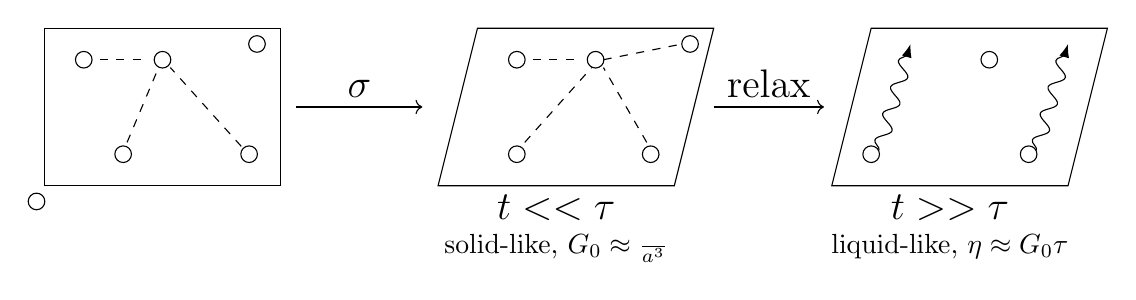
\begin{tikzpicture}
        \draw (-9,0) rectangle (-6,2);
        \draw (-8.5,1.6) circle (3pt);
        \draw[dashed] (-8.3,1.6) -- (-7.7,1.6);
        \draw (-7.5,1.6) circle (3pt);
        \draw (-6.3,1.8) circle (3pt);
        \draw (-9.1,-0.2) circle (3pt);
        \draw (-8,0.4) circle (3pt);
        \draw[dashed] (-7.95,0.55) -- (-7.55,1.5);
        \draw (-6.4,0.4) circle (3pt);
        \draw[dashed] (-6.5,0.5) -- (-7.4,1.5);
        \draw[->] (-5.8,1) -- (-4.2,1) node[anchor=south,midway] {\Large $\sigma$};

        \draw (-4,0) -- (-1,0) node[anchor=north,midway,align=center] {\Large $t << \tau$ \\ solid-like, $G_0 \approx \frac{\e}{a^3}$} -- (-0.5,2) -- (-3.5,2) -- cycle;
        \draw (-3,1.6) circle (3pt);
        \draw[dashed] (-2.8,1.6) -- (-2.2,1.6);
        \draw (-2,1.6) circle (3pt);
        \draw (-0.8,1.8) circle (3pt);
        \draw (-3,0.4) circle (3pt);
        \draw[dashed] (-2.9,0.55) -- (-2.05,1.5);
        \draw (-1.3,0.4) circle (3pt);
        \draw[dashed] (-1.35,0.55) -- (-1.9,1.5);
        \draw[dashed] (-1.9,1.6) -- (-0.9,1.8);
        \draw[->] (-0.5,1) -- (0.9,1) node[anchor=south,midway] {\Large relax};

        \draw (1,0) -- (4,0) node[anchor=north,midway,align=center] {\Large $t >> \tau$ \\ liquid-like, $\eta \approx G_0\tau$} -- (4.5,2) -- (1.5,2) -- cycle;
        \draw (1.5,0.4) circle (3pt);
        \draw (3.5,0.4) circle (3pt);
        \draw (3,1.6) circle (3pt);
        \draw[-{Latex[length=1.7mm]},snake it] (1.6,0.45) -- (2,1.8);
        \draw[-{Latex[length=1.7mm]},snake it] (3.6,0.45) -- (4,1.8);
    \end{tikzpicture}\\
    \vspace{20pt}
    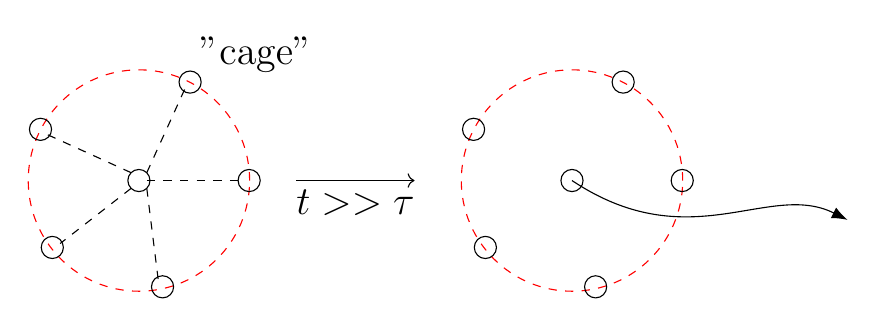
\begin{tikzpicture}
        \draw[red,dashed] (0,0) circle (40pt);
        \draw (1.4,0) circle (4pt);
        \draw[dashed] (0.1,0) -- (1.3,0);
        \draw (0,0) circle (4pt);
        \draw (0.65,1.25) circle (4pt) node[anchor=south west] {\Large "cage"};
        \draw[dashed] (0.1,0.1) -- (0.6,1.2);
        \draw (-1.25,0.65) circle (4pt);
        \draw[dashed] (-0.1,0.1) -- (-1.2,0.6);
        \draw (-1.1,-0.85) circle (4pt);
        \draw[dashed] (-0.1,-0.1) -- (-1,-0.8);
        \draw (0.3,-1.35) circle (4pt);
        \draw[dashed] (0.1,-0.1) -- (0.25,-1.3);

        \draw[->] (2,0) -- (3.5,0) node[anchor=north,midway] {\Large $t >> \tau$};
        \draw[red,dashed] (5.5,0) circle (40pt);
        \draw (6.9,0) circle (4pt);
        \draw (5.5,0) circle (4pt);
        \draw (6.15,1.25) circle (4pt);
        \draw (4.25,0.65) circle (4pt);
        \draw (4.4,-0.85) circle (4pt);
        \draw (5.8,-1.35) circle (4pt);
        \draw[-{Latex[length=2mm]}] (5.5,0) .. controls (7,-1) and (8,0) .. (9,-0.5);
    \end{tikzpicture}
\end{figure}
In this framework, the molecular explanation of the relaxation time $\tau$ is simply the time needed for an atom/molecule to escape the 'cage' formed by its nearest neighbours.
In other words, the time needed for the liquid to rupture the local (solid-like) order.
An atom/molecule vibrates within its cage due to thermal energy.
The frequency of vibration $\nu$ can be seen as the number of attempts made by the atom/molecule to escape the cage.
Taking into account the temperate $T$ and the escape energy barrier $\e$, it is possible to estimate $\tau$:
\begin{equation}
    \text{Prob to escape, } P \approx \frac{1}{\tau} = \nu \exp\left(-\frac{\e}{k_BT}\right).
\end{equation}
Practically, $\e$ can be estimated from the latent vaporisation energy of the liquid $\e_l$ with typically $\e \approx 0.4\e_l$.
The vibrations frequency is comparable to that of solids.
This gives relaxation times of $\tau = 10^{-12} \to 10^{-10}$s in simple liquids.
Such short times are experimentally not easily accessible and only the viscous behaviour is observed.
However, materials such as polymer melts can have relaxation times of seconds.
Putting the previous equations together, we get
\begin{equation}
    \eta = \frac{G_0}{\nu}\exp\left(\frac{\e}{k_BT}\right)
\end{equation}

\section{Liquids vs Glasses}
We have seen that the viscosity and the relaxation times of simple liquids vary exponentially with temperature, and with an activation energy that depends on the latent heat of vaporisation.
This model predicts that typical relaxation times remain in the range of pico- to nanoseconds for most temperature variations in liquids. \\
In reality, many liquids show a divergence of their relaxation time if they can be cooled to a low enough temperature without crystalising.
The molecules become 'kinetically trapped' in a liquid-like structural arrangement, but with a relaxation time so large (days, years) that the resulting material exhibits macroscopic properties of a solid.
This dramatic increase of relaxation time and hence viscosity can be modelled by the Vogel-Fulcher law:
\begin{figure}[H]
    \centering
    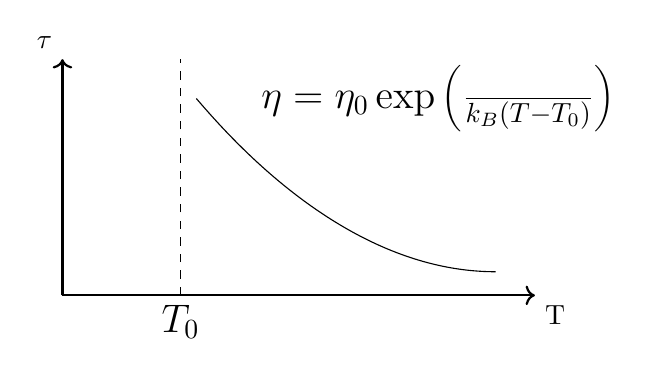
\begin{tikzpicture}
        \draw[thick,->] (0,0) -- (0,3) node[anchor=south east] {$\tau$};
        \draw[thick,->] (0,0) -- (6,0) node[anchor=north west] {T};
        \draw[dashed] (1.5,0) node[anchor=north] {\Large $T_0$} -- (1.5,3);
        \draw (5.5,0.3) parabola (1.7,2.5) node[anchor=west,xshift=20pt] {\Large $\eta = \eta_0\exp\left(\frac{\e}{k_B(T-T_0)}\right)$};
    \end{tikzpicture}
\end{figure}
Typical examples of glasses: oxides (windows), polymer glasses, metallic glasses.

Pitch can be seen as a very high viscosity liquid - $\eta_{\textit{pitch}} \approx 2.3\times10^{11}\eta_{\textit{water}}$.
There are about 100 months in between drops.
\emph{See the wikipedia article on the people who are sad enough to make this their life.}

The transition between a liquid state and a glass as the temperature decreases is called \textbf{the glass transition.}
Experimentally, it can be directly observed through discontinuities in some of the thermodynamics quantities.
It is however not a true thermodynamics transition because a glass is a kinetically trapped state and hence by definition not at thermodynamic equilibrium.
The question of the flow properties of glass remains controversial though.
The temperature at which the transition occurs is the \textbf{glass transition temperature.}
\begin{figure}[H]
    \centering
    \begin{tikzpicture}
        \draw[thick,->] (0,0) -- (0,6) node[anchor=south east] {$V_m = \frac{1}{\rho}$};
        \draw[thick,->] (0,0) -- (10,0) node[anchor=north west] {T};

        \draw[blue] (10,6) -- (6,10/3);
        \draw[dashed,blue] (6,10/3) -- (6,0) node[anchor=north] {\Large $T_m$};
        \draw[blue] (6,5/3) -- (2,5/6) node[anchor=south east,xshift=5pt] {\large solid};

        \draw[red] (6,10/3) -- (5,8/3);
        \draw[red,dashed] (5,8/3) -- (5,0) node[anchor=north] {\Large $T_{g_1}$};
        \draw[red] (5,8/3) -- (1.5,6/3) node[anchor=south east] {\large glass 1};

        \draw[green] (5,8/3) -- (4,2);
        \draw[green,dashed] (4,2) -- (4,0) node[anchor=north] {\Large $T_{g_2}$};
        \draw[green] (4,2) -- (1,1.4) node[anchor=south east,xshift=10pt] {\large glass 2};
    \end{tikzpicture}
\end{figure}
The glass transition temperature depends on the \textbf{rate} at which the cooling experiment is done.
This is not surprising given the fact that the glass transition is a kinetic effect.
If the experiment is carried out at a \textit{slower} cooling rate, the resulting transition temperature, $T_g$, will be lower.
Intuitively, this is because we leave more time for the molecule to rearrange as the temperature change occurs, hence hitting this 'jammed' state later.
The transition temperature cannot however be brought arbitrarily low.
The limit, called the \textit{Kuzmann temperature} is reached when the supercooled liquid has the same entropy as that of the equivalent crystaline solid.

\chapter{Basics of thermodynamics and application to surfaces and interfaces}
\section{Outline}
\begin{itemize}
    \item Basic reminder of thermodynamics $\to G,\mu$
    \item Thermodynamics of surfaces and interfaces
        \begin{itemize}
            \item Basic definitions
            \item Dupri equation
            \item Young equation
        \end{itemize}
\end{itemize}
Important concepts:
\begin{table}[H]
    \centering
    \begin{tabular}{c|c|c}
        & Solids & Liquids \\
        \hline
        Macro & elastic: $\sigma = Ge$ & viscous: $\sigma = \eta\dot{e}$ \\
        Micro & bond energy, $\e$ & escape prob from "cage"
    \end{tabular}
\end{table}
\begin{itemize}
    \item viscoelastic, $\sigma = \eta(\dot{e})\dot{e}$
    \item Glasses vs Liquids
\end{itemize}

\section{Basic thermodynamics reminder: Gibbs free energy, chemical potential, and phase diagrams}
This thermodynamics reminder aims at refreshing some of the basic concepts used in Soft Condensed Matter, but it assumes that the material has already be seen in details during previous lectures (Thermodynamics, 2B).
Many of the results are hence given without any demonstration.

\begin{enumerate}
    \item If \textbf{T and p are constant},the Gibbs free energy $G$ of a system determines the outcome of a process.
        This is a direct consequences of the second principle which states the entropy of an isolated system never decreases: \\
        For an isolated system and surroundings, for any process:
        \begin{align}
            \Delta S_{sys} &+ \Delta S_{surr} \geq 0 \\
            \Delta S_{sys} &- \frac{Q}{T} \geq 0, ~ p = \text{cst} \to Q = \Delta H \\
            T\Delta S_{sys} &- \Delta H \geq 0 \\
            \Delta G &\equiv \Delta H - T\Delta S_{sys} \leq 0
        \end{align}
        This is Gibss free energy.\\
        If $p=$cst, and $T=$cst:
        \begin{itemize}
            \item $\Delta G < 0$ - spontaneous process
            \item $\Delta G = 0$ - equilibrium
            \item $\Delta G > 0$ - disfavoured
        \end{itemize}
    \item The Gibbs free energy is related to the chemical potential.
        \begin{align}
            U &= TS - pV + \sum_i \mu_iN_i, \mu_i = \frac{G_i}{N_i} \\
            G &= U + pV - TS = H - TS \\
              &= \sum_i\mu_iN_i \\
            dG &= V\cancel{dp} - S\cancel{dT} + \sum_i\mu_i\,dN_i
        \end{align}
        The index $i$ designates speck(?) $i$.
        $\sum_i N_i = N$, total number of molcules.
        $\sum_i G_i = G$, total Gibbs free energy.
        $\mu_i$, partial Gibbs free energy per molecule $i$.
        Notation: $\bar{G}$, average Gibbs free energy per molecule (if $i=1,~\bar{G} = \mu$)/
    \item The chemical potential decreases with $T$ and increases with $p$.
        Since the intensive variables of coexisting phases are all equal at equilibrium, the chemical potential can be used to determine the phase behaviour of a system:
        \begin{align}
            d\mu &= \left(\frac{\p\mu}{\p T}\right)_p\,dT = -\bar{S}\,dT & d\mu &= \left(\frac{\p\mu}{\p p}\right)_T\,dp = \bar{V}\,dp,~ \bar{V} = \frac{1}{p}
        \end{align}
        \begin{multicols}{2}
            \begin{figure}[H]
                \centering
                \begin{tikzpicture}
                    \draw[thick,->] (0,0) -- (0,6) node[anchor=south east] {$\mu$};
                    \draw[thick,->] (0,0) -- (6,0) node[anchor=north west] {T};
                    \draw[blue] (0.5,4) -- (5.5,3) node[anchor=south west] {liquid};
                    \draw[green] (0.5,6) node[anchor=west] {vapour} -- (5.9,0.5);
                    \draw[red] (0.5,3.9) -- (2.9,3.4) -- (5.75,0.5);
                    \draw[red,dashed] (2.9,3.4) -- (2.9,0) node[anchor=north] {$T_V$};
                \end{tikzpicture}
            \end{figure}
            \columnbreak
            \begin{figure}[H]
                \centering
                \begin{tikzpicture}
                    \draw[thick,->] (0,0) -- (0,6) node[anchor=south east] {$\mu$};
                    \draw[thick,->] (0,0) -- (6,0) node[anchor=north west] {p};
                    \draw[blue] (0.5,2.5) -- (5.5,4) node[anchor=west] {liquid};
                    \draw[red] (0.5,0.5) -- (3,3.1) -- (5.5,3.8);
                    \draw[red,dashed] (3,3.1) -- (3,0) node[anchor=north] {$p_t$};
                    \draw[green] (0.4,0.5) -- (3.1,3.3) -- (5.5,5) node[anchor=south] {vapour};
                \end{tikzpicture}
            \end{figure}
        \end{multicols}
        \emph{Side note:} Solid/liquid/gas phase transitions are \textbf{first order} transitions, characterised by a discontinuity in density $\rho$ and in entropy.
        By definition of first order transitions, this is a discontinuity on the \textit{first derivative of the free energy.}
\end{enumerate}

\section{Thermodynamics of surfaces and interfaces}
Surfaces and interfaces play a fundamental role in soft matter.
For example, the surface energy of a given material determines the stability and reactivity of its surface.
The interfacial energy controls processes such as the self-assembly of complex structures and the mixing of two different liquids. \\
As for most problems in soft matter, it is helpful to start at the molecular level in order to identify the key physics concepts that will enable us to model the nature and properties of surfaces and interfaces.
A \textbf{surface} is by definition a topological defect.
It is the region of a medium where the atomic/molecular bonds are under-coordinated.
\begin{figure}[H]
    \centering
    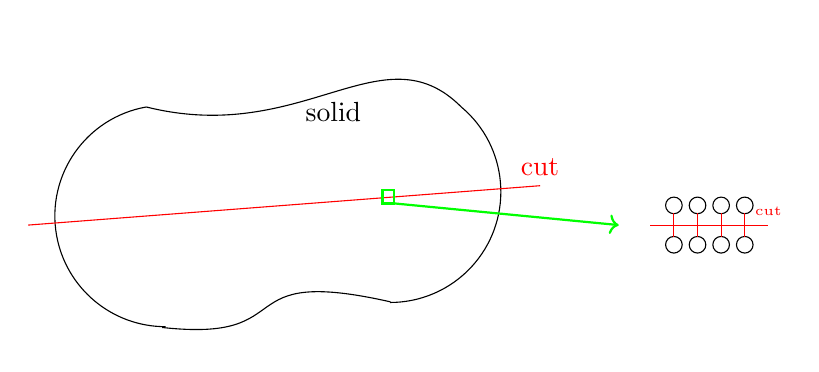
\begin{tikzpicture}
        \draw (-5,0) arc (100:270:40pt);
        \draw (-5,0) .. controls (-3,-0.5) and (-2,1) .. (-1,0) node[anchor=north,midway] {solid};
        \draw (-1,0) arc (50:-90:40pt);
        \draw (-4.8,-2.8) .. controls (-3,-3) and (-4,-2) .. (-1.9,-2.475);
        \draw[red] (-6.5,-1.5) -- (0,-1) node[anchor=south] {cut};
        \draw[green,->,thick] (-1.85,-1.225) -- (1,-1.5);
        \draw[green,thick] (-2,-1.225) rectangle (-1.85,-1.05);
        \draw (1.7,-1.25) circle (3pt);
        \draw (2.0,-1.25) circle (3pt);
        \draw (2.3,-1.25) circle (3pt);
        \draw (2.6,-1.25) circle (3pt);
        \draw (1.7,-1.75) circle (3pt);
        \draw (2,-1.75) circle (3pt);
        \draw (2.3,-1.75) circle (3pt);
        \draw (2.6,-1.75) circle (3pt);
        \draw[red] (1.4,-1.5) -- (2.9,-1.5) node[anchor=south] {\tiny cut};
        \draw[red] (1.7,-1.65) -- (1.7,-1.35);
        \draw[red] (2,-1.65) -- (2,-1.35);
        \draw[red] (2.3,-1.65) -- (2.3,-1.35);
        \draw[red] (2.6,-1.65) -- (2.6,-1.35);
    \end{tikzpicture}
\end{figure}
The under-coordinated bonds induce an excess of free energy to the system.
\begin{equation}
    dG_{surf} = \gamma\,dA,~ \gamma:\text{ surface energy (broken bonds) }\left[\frac{J}{m^2}\right]
\end{equation}
The proportionality factor $\gamma$ is called the surface free energy or simple the \textit{surface energy.}
It corresponds to half the \textbf{reversible} work that is needed to create a surface of unit area at constant temperature and pressure, without allowing for rearrangement of molecules or atoms.
\begin{figure}[H]
    \centering
    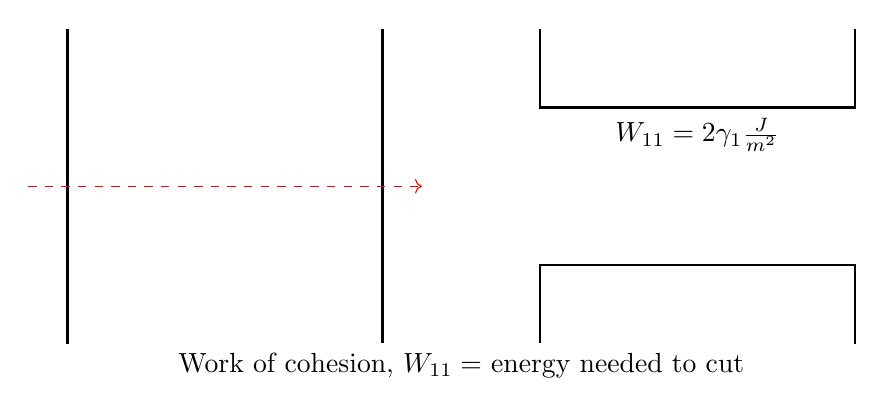
\begin{tikzpicture}
        \draw[thick] (-5,-2) -- (-5,2);
        \draw[thick] (-1,-2) -- (-1,2);
        \draw[red,dashed,->] (-5.5,0) -- (-0.5,0);
        \draw[thick] (1,2) -- (1,1) -- (5,1) node[anchor=north,midway] {$W_{11} = 2\gamma_1\frac{J}{m^2}$} -- (5,2);
        \draw[thick] (1,-2) -- (1,-1) -- (5,-1) -- (5,-2);
        \draw[white] (-4,-2) -- (4,-2) node[anchor=north,midway,black] {Work of cohesion, $W_{11} =$ energy needed to cut};
    \end{tikzpicture}
\end{figure}
In reality, the newly formed surface will tend to rearrange in order to minimise its surface energy.
Surfaces of solids will tend to reconstruct while molecules near the surface of a liquid will re-arrange.
Furthermore, pure surfaces are very rare (e.g. the surface of a solid in ultra-high vacuum).
It is therefore more useful to consider \textit{interfaces.}
We can extend the definition of surface energy to the interface between two media:
\begin{figure}[H]
    \centering
    \begin{tikzpicture}
        \draw[blue,thick] (-5,5) node[style={circle, draw=blue!60, thick, inner sep=0pt, minimum size=10pt},anchor=west,xshift=5pt] {1} -- (-5,3) node[anchor=east,black] {(i)} -- (-1,3) -- (-1,5);
        \draw[red,thick] (-5,1) -- (-5,2.9) node[style={circle, draw=red!60, thick, inner sep=0pt, minimum size=10pt},anchor=north west,xshift=5pt,yshift=-5pt] {2} -- (-1,2.9) -- (-1,1);

        \draw[blue,thick] (-5,-1) node[style={circle, draw=blue!60, thick, inner sep=0pt, minimum size=10pt},anchor=west,xshift=5pt] {1} -- (-5,-3) -- (-1,-3) -- (-1,-1);
        \draw[red,thick] (-5,-5.5) -- (-5,-3.5) node[style={circle, draw=red!60, thick, inner sep=0pt, minimum size=10pt},anchor=north west,xshift=5pt,yshift=-5pt] {2} -- (-1,-3.5) -- (-1,-5.5);
        \draw[white] (-5,-3) -- (-5,-3.5) node[anchor=east,black,midway] {(ii)};

        \draw[blue,thick] (1,5) node[style={circle, draw=blue!60, thick, inner sep=0pt, minimum size=10pt},anchor=west,xshift=5pt] {1} -- (1,3) -- (2,3);
        \draw[blue,thick,dashed] (2,3) -- (5,3);
        \draw[blue,thick] (5,3) node[anchor=west,black] {(iv)} -- (5,5);
        \draw[red,thick] (1,1) -- (1,2.9) node[style={circle, draw=red!60, thick, inner sep=0pt, minimum size=10pt},anchor=north west,xshift=5pt,yshift=-5pt] {2} -- (2,2.9);
        \draw[red,thick,dashed] (2,2.9) -- (5,2.9);
        \draw[red,thick] (5,2.9) -- (5,1);

        \draw[blue,thick] (1,-1) node[style={circle, draw=blue!60, thick, inner sep=0pt, minimum size=10pt},anchor=west,xshift=5pt] {1} -- (1,-3) -- (2,-3);
        \draw[blue,thick,dashed] (2,-3) -- (5,-3);
        \draw[blue,thick] (5,-3) -- (5,-1);
        \draw[red,thick] (1,-5.5) -- (1,-3.5) node[style={circle, draw=red!60, thick, inner sep=0pt, minimum size=10pt},anchor=north west,xshift=5pt,yshift=-5pt] {2} -- (2,-3.5);
        \draw[red,thick,dashed] (2,-3.5) -- (5,-3.5);
        \draw[red,thick] (5,-3.5) -- (5,-5.5);
        \draw[white] (5,-3) -- (5,-3.5) node[anchor=west,black,midway] {(iii)};

        \draw[->] (-0.5,3) -- (0.5,3);
        \draw[->] (-0.5,-3.25) -- (0.5,-3.25);
        \draw[->] (-3,0.5) -- (-3,-0.5);
        \draw[->] (3,-0.5) -- (3,0.5);
    \end{tikzpicture}
\end{figure}
By inspection, we can write
\begin{align}
    \underbrace{W_{12}A}_{(i)\to(ii)} + \underbrace{\Delta A\gamma_1 + \Delta A\gamma_2}_{(ii)\to(iii)} - \underbrace{W_{12}(A+\Delta A)}_{(iii)\to(iv)} = \underbrace{\gamma_{12}\Delta A}_{(i)\to(iv)}
\end{align}
This leads to the definition of the interfacial energy of the \textit{Dupr\'{e}} equation:
\begin{equation}
    \gamma_{12} = \gamma_1 + \gamma_2 - W_{12}
\end{equation}
where $\gamma_{12}$ is the interfacial energy, $\gamma_1$ and $\gamma_2$ the surface energies of the two media and $W_{12}$ the reversible \textit{work of adhesion} between both media.
The work of adhesion is literally the work necessary to separate the two media.
Intuitively, it represents the adhesion energy between both media.
This adhesion reduces the energy cost for creating the interfact because it partially compensates for the under-coordinated bonds of both surfaces.
\textbf{The sign of the work of adhesion is hence opposite that of the interfacial energy.}
In words, the Dupr\'{e} equation tells us that the free energy of an interface between two media is simply the energy necessary to create the surfaces of both media in a vacuum, minus the work needed to pull both media apart.

\section{Generalisation of the Dupr\'{e} equation}
The considerations that allowed us to deduce the Dupr\'{e} equation can easily be extended to more complicated interfaces, for example if two media are immersed in a third medium:
\begin{figure}[H]
    \centering
    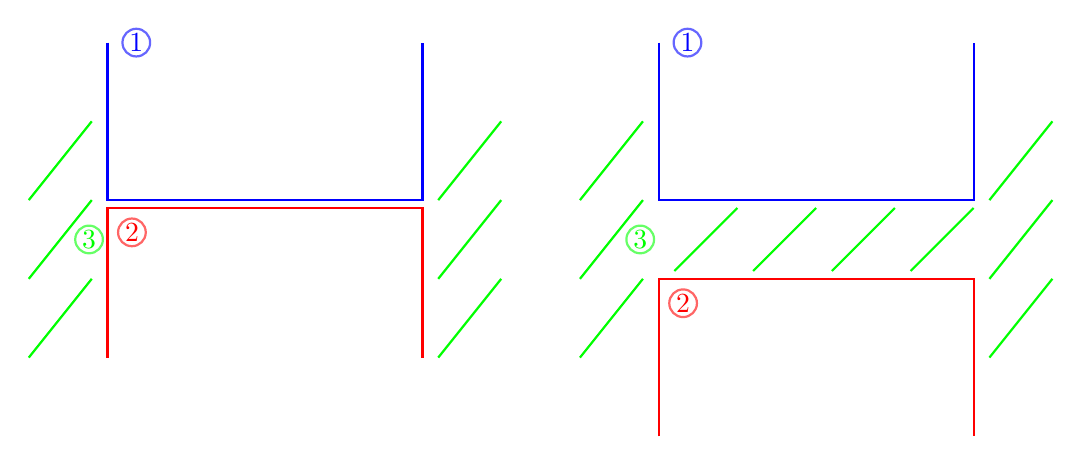
\begin{tikzpicture}
        \draw[blue,thick] (-5,5) node[style={circle, draw=blue!60, thick, inner sep=0pt, minimum size=10pt},anchor=west,xshift=5pt] {1} -- (-5,3) -- (-1,3) -- (-1,5);
        \draw[red,thick] (-5,1) -- (-5,2.9) node[style={circle, draw=red!60, thick, inner sep=0pt, minimum size=10pt},anchor=north west,xshift=5pt,yshift=-5pt] {2} -- (-1,2.9) -- (-1,1);

        \draw[blue,thick] (2,5) node[style={circle, draw=blue!60, thick, inner sep=0pt, minimum size=10pt},anchor=west,xshift=5pt] {1} -- (2,3) -- (6,3) -- (6,5);
        \draw[red,thick] (2,0) -- (2,2) node[style={circle, draw=red!60, thick, inner sep=0pt, minimum size=10pt},anchor=north west,xshift=5pt,yshift=-5pt] {2} -- (6,2) -- (6,0);

        \draw[thick,green] (-6,1) -- (-5.2,2);
        \draw[thick,green] (-6,2) -- (-5.2,3) node[style={circle, draw=green!60, thick, inner sep=0pt, minimum size=10pt},anchor=west,xshift=5pt,midway] {3};
        \draw[thick,green] (-6,3) -- (-5.2,4);
        \draw[thick,green] (-0.8,1) -- (-0,2);
        \draw[thick,green] (-0.8,2) -- (-0,3);
        \draw[thick,green] (-0.8,3) -- (-0,4);

        \draw[thick,green] (1,1) -- (1.8,2);
        \draw[thick,green] (1,2) -- (1.8,3) node[style={circle, draw=green!60, thick, inner sep=0pt, minimum size=10pt},anchor=west,xshift=5pt,midway] {3};
        \draw[thick,green] (1,3) -- (1.8,4);
        \draw[thick,green] (6.2,1) -- (7,2);
        \draw[thick,green] (6.2,2) -- (7,3);
        \draw[thick,green] (6.2,3) -- (7,4);
        \draw[thick,green] (2.2,2.1) -- (3,2.9);
        \draw[thick,green] (3.2,2.1) -- (4,2.9);
        \draw[thick,green] (4.2,2.1) -- (5,2.9);
        \draw[thick,green] (5.2,2.1) -- (6,2.9);
    \end{tikzpicture}
\end{figure}
\begin{equation}
    W_{132} = \gamma_{13} + \gamma_{23} - \underbrace{\gamma_{12}}_{\gamma_1 + \gamma_2 - W_{12} \cdots}
\end{equation}
One of the most common situations where this occurs is for liquids droplets at the surface of a solid in air:
\begin{figure}[H]
    \centering
    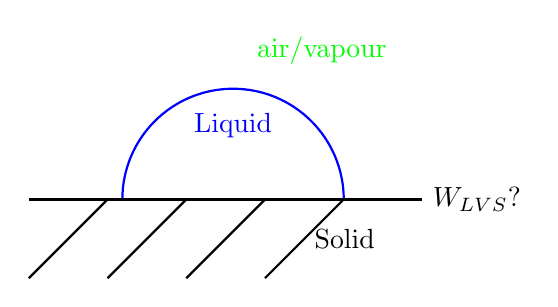
\begin{tikzpicture}
        \draw[thick,blue] (2,0) arc (0:180:40pt) node[anchor=north,midway,yshift=-5pt] {Liquid} node[anchor=south west,midway,xshift=5pt,yshift=5pt,green] {air/vapour};
        \draw[thick] (-2,0) -- (3,0) node[anchor=west] {$W_{LVS}$?};

        \draw[thick] (-2,-1) -- (-1,0);
        \draw[thick] (-1,-1) -- (0,0);
        \draw[thick] (0,-1) -- (1,0);
        \draw[thick] (1,-1) -- (2,0) node[anchor=west,midway] {Solid};
    \end{tikzpicture}
\end{figure}

\section{The Young Equation}
The surface energy of the liquid $\gamma$ (or liquid-vapour interface energy) is often referred to as \textit{surface tension} because it effectively acts as a force resisting deformations of the interface.
The work necessary to increase of decrease the surface of a drop by an area $dA$ is
\begin{equation}
    W = \gamma\,dA
\end{equation}
The fact that the liquid forms a spherical droplet reflects the system's minimisation of the interfacial energy between the liquid and the vapour.
The solid also influences the shape of the droplet t the solid-liquid interface.

At equilibrium, there exists an equation linking all the interfacial energies and the angle $\theta$ formed by the droplet with the solid.
This equation can be deduced from the cost of free energy needed to increase the contact area of the drop with the solid bt a value $dA$.
The solid-vapour contact area will decrease by $dA$ while the solid-liquid interface will increase by $dA$.
For small surface increments ($dA << A$), it is possible to show the the liquid-vapour area will increase by $dA\cos\theta$:
\begin{figure}[H]
    \centering
    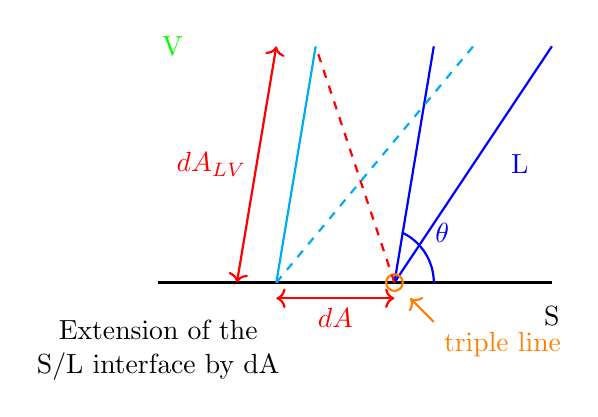
\begin{tikzpicture}
        \draw[thick] (-2,0) node[anchor=north,yshift=-10pt,align=center] {Extension of the \\ S/L interface by dA} -- (3,0) node[anchor=north,yshift=-5pt] {S};
        \draw[thick,blue] (1,0) -- (3,3) node[anchor=west,midway,xshift=10pt] {L};
        \draw[thick,blue] (1,0) -- (1.5,3);
        \draw[thick,orange] (1,0) circle (3pt);
        \draw[thick,orange,->] (1.5,-0.5) node[anchor=north west] {triple line} -- (1.2,-0.2);
        \draw[thick,blue] (1.5,0) arc (0:65:20pt) node[anchor=south west,midway] {$\theta$};
        \draw[red,dashed,thick] (1,0) -- (0,3);
        \draw[cyan,dashed,thick] (-0.5,0) -- (2,3);
        \draw[cyan,thick] (-0.5,0) -- (0,3);
        \draw[red,thick,<->] (-1,0) -- (-0.5,3) node[anchor=east,midway] {$dA_{LV}$} node[anchor=east,xshift=-30pt,green] {V};
        \draw[red,thick,<->] (1,-0.2) -- (-0.5,-0.2) node[anchor=north,midway] {$dA$};
    \end{tikzpicture}
\end{figure}
$\theta$ is the contact angle formed by the solid plane with tangent to the liquid/vapour interface at the triple line.
If we assume constant temperature, pressure and number of molecules, the change in free energy will be:
\begin{equation}
    dG = \sum_{i,j=S,L,V} \gamma_{ij}\,dA_{ij} = \gamma_{SL}\underbrace{dA_{SL}}_{dA} + \gamma_{SV}\underbrace{dA_{SV}}_{-dA} + \gamma_{LV}\underbrace{dA_{LV}}_{\sim dA\cos\theta} = 0
\end{equation}
At equilibrium, we must have $dG = 0$.
This is only always true of:
\begin{align}
    \gamma_{SL} - \gamma_{SV} + \gamma_{LV}\cos\theta = 0 \\
    \gamma_{LV}\cos\theta = \gamma_{SV} - \gamma_{SL}
\end{align}
This is the \textbf{Young equation.}\\
\textit{Side note:} It is often acceptable to use the approximation $\gamma_{SV} \approx \gamma_S$ and $\gamma_{LV} \approx \gamma_L$ leading to a simplified Young equation:
\begin{align}
    \gamma_{SV} &= \gamma_S + \underbrace{\gamma_V}_{<<\gamma_S} - \underbrace{W_{SV}}_{<<\gamma_S} \approx \gamma_S \\
    \gamma_{LV} &\approx \gamma_L,\text{ surface tension of liquid}
\end{align}

\chapter{Interfaces with solids: elasticity and surface deformations}
\section{Outline}
\begin{itemize}
    \item Linear bulk deformation of solids (basics)
        \begin{itemize}
            \item moduli
            \item Poisson ratio
        \end{itemize}
    \item Elastic surface deformation (indentation)
        \begin{itemize}
            \item Hertz model
            \item JKR model
        \end{itemize}
\end{itemize}

Important concepts from last lecture:
\begin{itemize}
    \item Thermodynamics reminder: $G,\mu$ (p,T constants)
    \item Surface energy, $\frac{J}{m^2} \leftrightarrow$ Interface energy $\frac{J}{m^2}$
        \begin{equation*}
            \text{Medium X } \to \gamma_x \leftrightarrow \frac{\text{Medium X}}{\text{Medium Y}} \to \gamma_{xy}
        \end{equation*}
    \item Dupr\'{e} equation
        \begin{equation}
            \gamma_{xy} = \gamma_x + \gamma_y - W_{xy}
        \end{equation}
        where $W_{xy}$ is the work of adhesion
    \item Young equation
        \begin{equation}
            \gamma_{LS} + \gamma_{LV}\cos\theta - \gamma_{SV} = 0
        \end{equation}
        \begin{figure}[H]
            \centering
            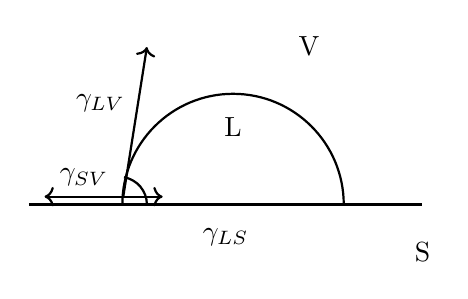
\begin{tikzpicture}
                \draw[thick] (2,0) arc (0:180:40pt) node[anchor=north,midway,yshift=-5pt] {L} node[anchor=south west,midway,xshift=20pt,yshift=10pt] {V};
                \draw[thick] (-2,0) -- (3,0) node[anchor=north,yshift=-10pt] {S} node[anchor=north,midway,yshift=-5pt] {$\gamma_{LS}$};
                \draw[thick] (-0.5,0) arc (0:80:10pt);
                \draw[thick,->] (-0.8,0.1) -- (-0.3,0.1);
                \draw[thick,->] (-0.8,0.1) -- (-0.5,2) node[anchor=south east,midway] {$\gamma_{LV}$};
                \draw[thick,->] (-0.8,0.1) -- (-1.8,0.1) node[anchor=south,midway] {$\gamma_{SV}$};
            \end{tikzpicture}
        \end{figure}
\end{itemize}

\section{Elasticity of solids}
We have seen in previous lectures that typical solids deform elastically when small stresses are applied.
This is the basis of Hook's law and defines the concept of \textit{'Hookean solids'.}
While straightforward in axisymmetric or 1-dimensional systems (e.g. a spring), the stress induced by an applied strain can have components in multiple directions not necessarily related to that of the applied strain.
Providing a general description to the elastic deformation of solids requires \textit{tensorial} analysis.
For our purpose, we can think of a tensor as a multidimensional array of components (e.g. a matrix for in the case of a standard 2-dimensional array).
Tensors obey certain transformation rules, for example between different referential systems, and be of any dimension (the dimension is called the 'rank').

\begin{example}[The Stress Tensor]
For a simple illustration, we can consider an arbitrary strain applied to a cube in a reference frame $X_1,X_2,X_3$.
The strain will result in a stress that can be measured in many different directions.
These measurements define the second rank stress tensor.

\begin{multicols}{2}
    \begin{figure}[H]
        \centering
        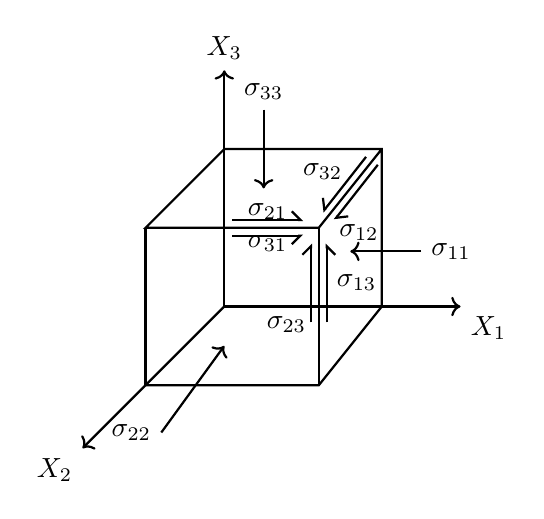
\begin{tikzpicture}
            \draw[thick,->] (0,0) -- (0,3) node[anchor=south] {$X_3$};
            \draw[thick,->] (0,0) -- (3,0) node[anchor=north west] {$X_1$};
            \draw[thick,->] (0,0) -- (-1.8,-1.8) node[anchor=north east] {$X_2$};
            \draw[thick] (-1,-1) -- (1.2,-1) -- (2,0) -- (2,2) -- (0,2) -- (-1,1) -- (1.2,1) -- (2,2);
            \draw[thick] (-1,-1) -- (-1,1);
            \draw[thick] (1.2,-1) -- (1.2,1);
            \draw[thick,->] (0.5,2.5) node[anchor=south] {$\sigma_{33}$} -- (0.5,1.5);
            \draw[thick,->] (2.5,0.7) node[anchor=west] {$\sigma_{11}$} -- (1.6,0.7);
            \draw[thick,->] (-0.8,-1.6) node[anchor=east] {$\sigma_{22}$} -- (0,-0.5);
            \draw[-{Straight Barb[left]},thick] (0.1,1.1) -- (1,1.1) node[anchor=north,midway,yshift=-2pt] {$\sigma_{31}$};
            \draw[-{Straight Barb[right]},thick] (0.1,0.9) -- (1,0.9) node[anchor=south,midway,yshift=2pt] {$\sigma_{21}$};
            \draw[-{Straight Barb[right]},thick] (1.8,1.9) -- (1.25,1.2) node[anchor=south east,midway,xshift=3pt,yshift=-2pt] {$\sigma_{32}$};
            \draw[-{Straight Barb[left]},thick] (1.95,1.8) -- (1.4,1.1) node[anchor=north west,yshift=2pt,xshift=-2pt] {$\sigma_{12}$};
            \draw[-{Straight Barb[left]},thick] (1.1,-0.2) -- (1.1,0.8) node[anchor=east,midway,yshift=-15pt,xshift=2pt] {$\sigma_{23}$};
            \draw[-{Straight Barb[right]},thick] (1.3,-0.2) -- (1.3,0.8) node[anchor=west,midway] {$\sigma_{13}$};
        \end{tikzpicture}
    \end{figure}
    \columnbreak
    \begin{equation}
        \unl{\sigma} = \begin{pmatrix} \sigma_{11} & \sigma_{12} & \sigma_{13} \\ \sigma_{21} & \sigma_{22} & \sigma_{23} \\ \sigma_{31} & \sigma_{32} & \sigma_{33} \end{pmatrix}
    \end{equation}
\end{multicols}
Notes:
\begin{itemize}
    \item The eigenvalues of $\sigma_{ij}$ are often represented as $\sigma_1,\sigma_2,\sigma_3$ and referred to as the principle stresses.
    \item A tensor is often underlined or written in bold font to avoid confusion with scalar quantities.
    \item The stress tensor is symmetric: $\sigma_{ij} = \sigma_{ji}$.
        Intuitively, this can be understoof when considering the limiting case where the cube is infinitesimally small: the forces across each face are uniform and normal forces on opposite faces must hence be equal in magnitude and opposide in direction.
\end{itemize}
\end{example}
Similar to the stress tensor, $\unl{\sigma}$, we can define a second rank strain tensor $\unl{e}$, so that
\begin{equation}
    \unl{\sigma} = \unl{c}\unl{e}.
\end{equation}
Here $\unl{c}$ is the elastic stiffness.
In all generality, since $\unl{c}$ relates two second rank tensors, it must be a fourth rank tensor:
\begin{equation}
    \sigma_{ij} = c_{ijkl}e_{kl}
\end{equation}
In the 3D case, we should calculate $\sigma_{ij}$ as follows:
\begin{equation}
    \sigma_{11} = c_{1111}e_{11} + c_{1112}e_{12} + c_{1113}e_{13} + \cdots + c_{1132}e_{32} + c_{1133}e_{33}
\end{equation}
It is important to realise that in general, different directions are coupled: a stress applied in a single direction will generate strains in multiple directions.
If all $\sigma_{ij} = 0$ except for $\sigma_{11}$, we may still have most $e_{ij}\neq0$.
Reciprocally, a strain in a single direction may be coupled to stresses in many directions.
\begin{figure}[H]
    \centering
    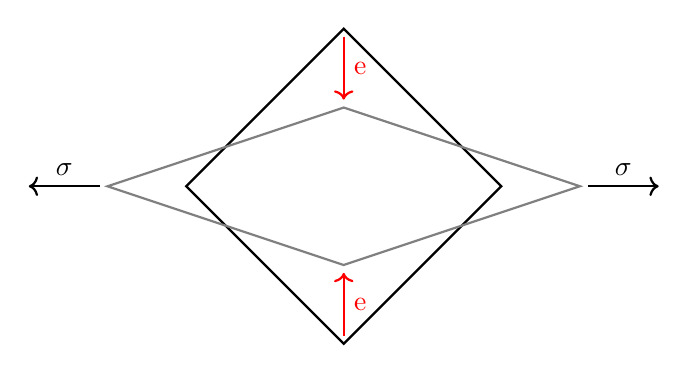
\begin{tikzpicture}
        \draw[thick] (-2,0) -- (0,2) -- (2,0) -- (0,-2) -- cycle;
        \draw[gray,thick] (-3,0) -- (0,1) -- (3,0) -- (0,-1) -- cycle;
        \draw[red,thick,->] (0,1.9) -- (0,1.1) node[anchor=west,midway] {e};
        \draw[red,thick,->] (0,-1.9) -- (0,-1.1) node[anchor=west,midway] {e};
        \draw[thick,->] (3.1,0) -- (4,0) node[anchor=south,midway] {$\sigma$};
        \draw[thick,->] (-3.1,0) -- (-4,0) node[anchor=south,midway] {$\sigma$};
    \end{tikzpicture}
\end{figure}

\section{Basic relationship between compression and shear}
The fact that, for a solid, strain and stress are generally coupled between different directions has some consequences when deriving the solids' compression modulus (called Young Modulus, $E$), and the Shear Modulus, $G$.
For a homoegeneous solid, a relationship between the Young and Shear moduli can be derived easily by comparing the deformation of a cube in two different referential.
We find:
\begin{equation}
    E = 2G(1+\nu)
\end{equation}
We have used the so-called \textbf{Poisson ratio} $\nu$ that quantifies how much a compression applied in a given direction can induce a compression or traction in a perpendicular direction.
Similarly, we can relate the Young modulus to the so-called Bulk modulus of elasticity $K$ which relates the volumetric stress to the volumetric strain.
We find:
\begin{equation}
    K = \frac{E}{3(1-2\nu)}
\end{equation}

\section{The Poisson Ratio}
The Poisson effect is the phenomenon by which a material tends to expand (respectively compress) in directions perpendicular to the direction of compression (respectively extension).
The Poisson ratio quantifies the magnitude of this effect for a given material; it is \textit{the ratio of transverse strain to axial strain.}
The Poisson effect comes from the simple fact that for any given finite object, a compression in a given direction must induce a perpendicular extension in order to conserve the volume occupied by the object.
In reality, the volume of the object deformed is only perfectly conserved if its Poisson ratio is $\nu = \frac12$.
From the last equation, it is immediately obvious that the bulk modulus of a material diverges is $\nu = \frac12$.
\begin{equation}
    K = \frac{E}{3(1-2\nu)} \to_{\nu\to\frac12} \infty
\end{equation}
When a material has a Poisson ratio of $\nu=\frac12$, it is considered \textbf{incompressible.}
In reality, most materials are compressible and their volume can change under stress through elastic deformation of inter-molecular or atomic bonds, leading to a smaller Poisson ratio value (e.g. deep-sea technology).
The Poisson ratio can however also take negative values for certain materials and composites.
In all generality, we have
\begin{equation}
    -1 < \nu < \frac12
\end{equation}
\begin{itemize}
    \item For most homoegeneous and isotropic solids, the Poisson ratio satisfies $0 < \nu < \frac12$.
        This means that, for most homogeneous and isotropic solids (e.g. crystals, metals), a compression applied in a given direction will induce some extension in the perpendicular direction, at least to some extent.
    \item Materials that are not homoegeneous in the sense that they exhibit some mesoscale structure (e.g. fibres, nanostructured solids) or composite materials (foams, colloidal suspensions) can often take a broad range of Poisson ratio values depending on their precise structure.
        This is because the re-arrangement of the mesoscale structure under an external force can be highly anisotropic, depending on the details of the system.
    \item Particular classes of foams and flexible arrays of composite materials can be designed to exhibit a \textit{negative} Poisson ratio.
        This is however unusual and is due to the particular structure of the foam/array rather than the properties of its components.
\end{itemize}

\section{Axisymmetric surface deformations and effective values}
We have seen different moduli and the Poisson ratio characterise the properties of solids when deformed.
In most practical cases, the applied stress on a solid is not uniform but can be highly localised to certain regions of the solid's surface.
The simplest example is that of two solids pressed against each other.
\begin{figure}[H]
    \centering
    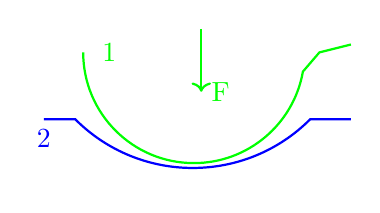
\begin{tikzpicture}
        \draw[green,thick] (-2,2) arc (180:350:40pt) node[anchor=south,xshift=-70pt] {1} -- (1,2) -- (1.4,2.1);
        \draw[blue,thick] (-2.5,1.15) node[anchor=north] {2} -- (-2.1,1.15) arc (225:315:60pt) -- (1.4,1.15);
        \draw[green,thick,->] (-0.5,2.3) -- (-0.5,1.5) node[anchor=west] {F};
    \end{tikzpicture}
\end{figure}
The localised contact point(s) will result in localised surface deformation of each solid.
Quantifying surface deformations is therefore very useful in soft matter and materials sceicne.
Practically, it is helpful to define effective quantities in abinary contact, e.g. the redued Young modulus, $E^*$:
\begin{equation}
    E^* = \left(\frac{1-\nu_1^2}{E_1} + \frac{1-\nu_2^2}{E_2}\right)^{-1}
\end{equation}
The reduced Young modulus represents an effective Young modulus for the whole contact when taking into account the Poisson ratio of each material.
$E^*$ effectively quantifies the combined deformation of both materials.
If one of the materials is much softer than the other, it will experience most of the deformation and $E^*$ then reflects almost exclusively the properties of the softer material:
\begin{equation}
    E_1 >> E_2 \implies E^* \approx \frac{E_1}{1-\nu_1^2}
\end{equation}

\section{The Hertz Model}
Since most contacts are not flat, it is convenient and general to assume a spherical indenter of radius $R_1$ compressing a spherical surface with a radius of curvature $R_2$.
If $R_2 = \infty$, then the indented surface is flat, a particular case of the more general model.
Similarly to our definition of the reduced Young modulus $E^*$, it is useful to define an effective contact radius for the deformation, or the reduced contact radius, $R^*$:
\begin{equation}
    \frac{1}{R^*} = \frac{1}{R_1} + \frac{1}{R_2}
\end{equation}
In 1882, Hertz derived an equation for the contact radius between the spheres:
\begin{equation}
    a^3 = \frac{3F_LR^*}{4E^*}
\end{equation}
He demonstrated the penetration depth for a given applied force load $F_L$ is given by:
\begin{equation}
    \delta = \frac{a^2}{R^*} =  \left(\frac{9R_L^2}{16E^{*2}R^*}\right)^{1/3},~ F_L = \frac43 E^*\sqrt{R^*} \delta^{3/2}
\end{equation}
The Hertz model remains to date the benchmark used for calculating forces and elasticities in indentation problems, also in nanotechnology.
However, it is simplistic in the sense that it does not take into account any surface forces, for instance those leading to adhesion.

\section{Hertz model with adhesion: the JKR Theory}
Scientists have further extended the Hertz model to include adhesion forces between the two spheres, similarly to the approach used by Sneddon for the flat punch.
The most common theory is so-called Johnson-Kendall-Robert theory (JKR).
Other theories exist such as the DMT (Derjaguin-Muller-Toporov) and Maugis theories, each presenting different hypotheses about the local adhesive forces around the indentation area.
The JKR model assumes that the adhesion forces only operate within the contact area.
Using an approach similar to that of the flat punch development, it can be shown that the contact area varies as a function of the indentation force $F_L$ following:
\begin{equation}
    a^3 = \frac{3R^*}{4E^*}\left(F_L + 3\pi W_{adh}R^* + \sqrt{6\pi W_{adh}R^*F_L + (3\pi W_{adh}R^*)^2}\right)
\end{equation}
The indentation for a given contact area is then
\begin{equation}
    \delta = \frac{a^2}{R^*} - \sqrt{\frac{2\pi aW_{adh}}{E^*}}
\end{equation}
and the adhesion force is simply
\begin{equation}
    F_{adh} = -\frac32 \pi W_{adh}R^*
\end{equation}

\chapter{}
\section{Outline}
\begin{itemize}
    \item Young and Dupr\'{e} equations $\to$ wetting
    \item Capillary forces and surface tension
        \begin{itemize}
            \item spreading
            \item Laplace equation
                \begin{itemize}
                    \item Kelvin equation
                    \item solid particles at the surface of liquids
                \end{itemize}
        \end{itemize}
\end{itemize}

Important concepts from last lecture:
\begin{itemize}
    \item Linear bulk deformation of solids
        \begin{itemize}
            \item tensor, $\unl{c}$ - 4th rank
                \begin{equation}
                    \unl{\sigma} = \sigma_{ij},~ \unl{\sigma} = \unl{c}\unl{e}
                \end{equation}
            \item $E,G,\nu$
        \end{itemize}
    \item Surface forces of solids
    \item reduced Young modulus $E^*$
        \begin{itemize}
            \item Hertz model (no adhesion)
            \item JKR $+ W_{adh}$
        \end{itemize}
\end{itemize}

\section{The Young-Dupr\'{e} equation: quantifying wetting}
In previous lectures, thermodynamics provides a useful framework for describing and predicting the fate of surfaces and interfaces.
Assuming interfaces at equillibrium , we derived the following equation:
\begin{equation}
    \gamma_{12} = \gamma_1 + \gamma_2 - W_{12},~ 1,2 = S,L,V
\end{equation}
In the particular case of the drop of liquid on the surface of a solid in a gas, we found that at equilibrium, the different interfacial energies must satisfy:
\begin{equation}
    \gamma_{SV} = \gamma_{LV}\cos\theta + \gamma_{LS}
\end{equation}
\begin{figure}[H]
    \centering
    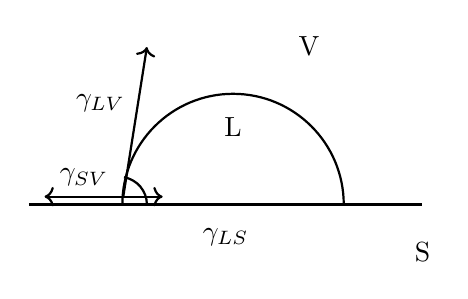
\begin{tikzpicture}
        \draw[thick] (2,0) arc (0:180:40pt) node[anchor=north,midway,yshift=-5pt] {L} node[anchor=south west,midway,xshift=20pt,yshift=10pt] {V};
        \draw[thick] (-2,0) -- (3,0) node[anchor=north,yshift=-10pt] {S} node[anchor=north,midway,yshift=-5pt] {$\gamma_{LS}$};
        \draw[thick] (-0.5,0) arc (0:80:10pt);
        \draw[thick,->] (-0.8,0.1) -- (-0.3,0.1);
        \draw[thick,->] (-0.8,0.1) -- (-0.5,2) node[anchor=south east,midway] {$\gamma_{LV}$};
        \draw[thick,->] (-0.8,0.1) -- (-1.8,0.1) node[anchor=south,midway] {$\gamma_{SV}$};
    \end{tikzpicture}
\end{figure}
We also used the approximation that the contribution from the gas is often negligible:
\begin{equation}
    \gamma_{LV} \approx \gamma_L,~ \gamma_{SV} \approx \gamma_S
\end{equation}
We can now combine the approximated \textit{Young equation} with the \textit{Dupr\'{e} equation} to get the so called \textit{Young-Dupr\'{e} equation}:
\begin{equation}
    \gamma_L (1+\cos\theta) = W_{SL}
\end{equation}
Although not formally correct, this equation is very useful because it relates the contact angle formed by a droplet at the surface of a solid to the surface tension of the liquid and the affinity of the liquid for the solid.
The \textbf{work of adhesion, $W_{SL}$,} hence quantifies the \textit{wetting} properties of the solid by the liquid in the droplet.
\begin{figure}[H]
    \centering
    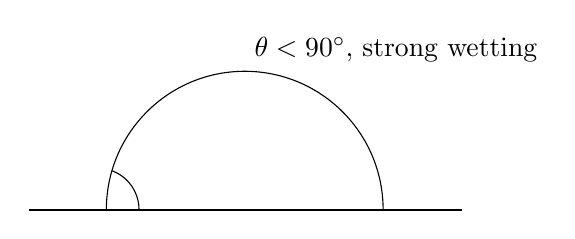
\begin{tikzpicture}
        \draw[thick] (-2.5,0) -- (3,0);
        \draw (2,0) arc (0:180:50pt) node[anchor=south west,midway] {$\theta < 90^{\circ}$, strong wetting};
        \draw (-1.1,0) arc (0:70:15pt);
    \end{tikzpicture}
    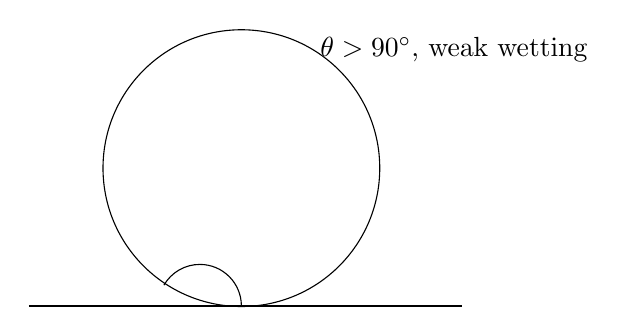
\begin{tikzpicture}
        \draw[thick] (-2.5,0) -- (3,0);
        \draw (0.2,1.75) circle (50pt) node[anchor=south west,yshift=35pt,xshift=25pt] {$\theta > 90^{\circ}$, weak wetting};
        \draw (0.2,0) arc (0:150:15pt);
    \end{tikzpicture}
\end{figure}
This equation is only rigorous for solvents that do not penetrate into the solid, and perfectly flat surfaces.
\begin{figure}[H]
    \centering
    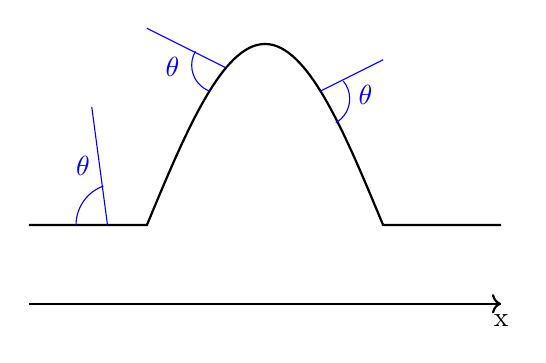
\begin{tikzpicture}
        \draw[thick,->] (-3,0) -- (3,0) node[anchor=north] {x};
        \draw[thick] (-3,1) -- (-1.5,1) sin (0,3.3) cos (1.5,1) -- (3,1);

        \draw[blue] (-2,1) -- (-2.2,2.5) node[anchor=east,midway] {$\theta$};
        \draw[blue] (-2.4,1) arc (180:110:15pt);

        \draw[blue] (-0.5,3) -- (-1.5,3.5) node[anchor=north,midway,xshift=-5pt] {$\theta$};
        \draw[blue] (-0.7,2.7) arc (250:150:10pt);

        \draw[blue] (0.7,2.7) -- (1.5,3.1) node[anchor=north,midway,xshift=5pt] {$\theta$};
        \draw[blue] (0.9,2.3) arc (-60:40:10pt);
    \end{tikzpicture}
    \begin{tikzpicture}
        \draw[thick,->] (0,0) -- (6,0) node[anchor=north] {x};
        \draw[thick,->] (0,0) -- (0,4);
        \draw (0.5,2) -- (1,2) sin (2,0.5) cos (3,2) sin (4,3.5) cos (5,2) -- (5.5,2);
    \end{tikzpicture}
\end{figure}
In order to take into account the roughness of 'real' surfaces, Robert Wenzel proposed a simple correction to the Young equation:
\begin{equation}
    \cos\theta_0 = \cos\theta\cdot r
\end{equation}
where $\theta_0$ is the observed angle and $r$ is the ration actual surface area over the ideal (perfectly flat) area.
In reality, more complicated effects can happen, especially if the surface of the solid presents some holes large enough to trap air.
In such case, Wenzel's correction is not sufficient and we have to use the Cassie equation:
\begin{figure}[H]
    \centering
    \begin{tikzpicture}
        \draw (-4.5,0) -- (-4,0) -- (-4,1) -- (-3.5,1) -- (-3.5,0) -- (-2.5,0) -- (-2.5,1) -- (-2,1) -- (-2,0) -- (-1,0) -- (-1,1) -- (-0.5,1) -- (-0.5,0) -- (0.5,0) -- (0.5,1) -- (1,1) -- (1,0) -- (1.5,0);
        \draw (-1.5,1.5) circle (20pt) node[anchor=north,yshift=10pt] {L};
        \draw[thick,->] (-1.5,-0.5) node[anchor=north] {trapped air} -- (-1.5,0.5);
        \draw[thick,<->] (-0.4,0.5) -- (0.4,0.5) node[anchor=north,midway] {$D_1$};

        \draw (2.5,0) -- (3,0) -- (3,1) -- (3.5,1) -- (3.5,0) -- (4.5,0) -- (4.5,1) -- (5,1) -- (5,0) -- (6,0) -- (6,1) -- (6.5,1) -- (6.5,0) -- (7.5,0) -- (7.5,1) -- (8,1) -- (8,0) -- (8.5,0) node[anchor=south,yshift=30pt] {$D_2 << D_1$};
        \draw (3.25,1) arc (180:0:42pt) node[anchor=north,midway,yshift=-10pt] {L};
        \draw[thick,<->] (6.6,0.5) -- (7.4,0.5) node[anchor=north,midway] {$D_2$};
    \end{tikzpicture}
\end{figure}
\begin{equation}
    \cos\theta_0 = rf\cos\theta + f - 1
\end{equation}
f is the fraction of the surface in contact with the liquid.
The transition between the Wenzel and Cassie regimes is not trivial, but plays an important role in nature, for example in the lotus-left effect (super-hydrophibicity).

\section{Spreading of liquid droplets}
Young equation can also be used to study liquid-liquid interfaces, for example when a drop of liquid is added to the interface between an immiscible liquid and a gas or a liquid-liquid interface:
\begin{figure}[H]
    \centering
    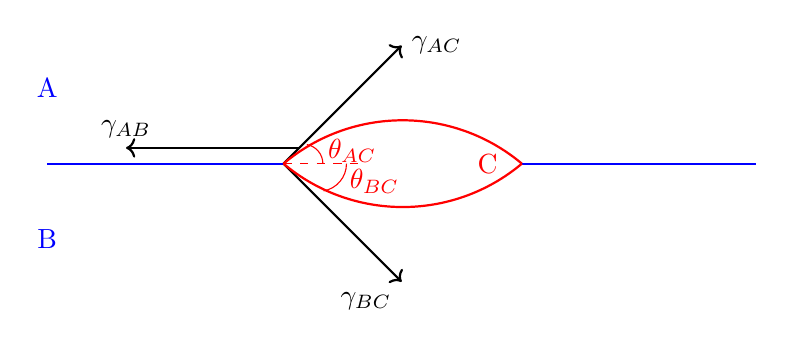
\begin{tikzpicture}
        \draw[blue,thick] (-4,0) node[anchor=north,yshift=-20pt] {B} node[anchor=south,yshift=20pt] {A} -- (-1,0) ;
        \draw[blue,thick] (2,0) -- (5,0);
        \draw[->,thick] (-1,0) -- (0.5,1.5) node[anchor=west] {$\gamma_{AC}$};
        \draw[->,thick] (-1,0) -- (0.5,-1.5) node[anchor=north east] {$\gamma_{BC}$};
        \draw[thick,->] (-0.8,0.2) -- (-3,0.2) node[anchor=south] {$\gamma_{AB}$};
        \draw[thick,red] (-1,0) arc (130:50:67pt);
        \draw[thick,red] (-1,0) arc (230:310:67pt) node[anchor=east,xshift=-5pt] {C};
        \draw[red,dashed] (-1,0) -- (0,0);
        \draw[red] (-0.5,0) arc (0:80:7pt) node[anchor=west,midway] {$\theta_{AC}$};
        \draw[red] (-0.2,0) arc (0:-80:10pt) node[anchor=west,midway] {$\theta_{BC}$};
    \end{tikzpicture}
\end{figure}
It is immediate from the figure that we can apply the same energy balance as we used for deriving the Young equation.
We can write
\begin{equation}
    \gamma_{AB} = \gamma_{AC}\cos\theta_{AC} + \gamma_{BC}\cos\theta_{BC}
\end{equation}oIf $\gamma_{AB} > \gamma_{AC}\cos\theta_{AC} + \gamma_{BC}\cos\theta_{BC}$, the balance of forces will elongate the droplet along the $AB$ interface until a balance of forces is re-established, thereby reducing $\theta_{AC}$ and $\theta_{BC}$.
It is easy to see at the limit where $\theta_{AC} = \theta_{BC} = 0$, the droplet is completely spread over the $AB$ interface and forms a film.
We can therefore define the \textbf{spreading coefficient} as follows:
\begin{equation}
    S_{ACB} = \gamma_{AB} - \gamma_{AC} - \gamma_{BC} \begin{cases} > 0 & \text{spreading} \\ < 0 & \text{lensing} \end{cases}
\end{equation}
The most common case is when $A$ is air, and $B$ and $C$ are two immiscible liquids such as oil and water, separated by gravity.
In this case, we can use the usual approximation for the Young equation (o: oil, w:water),
\begin{equation}
    S_{ow} = \gamma_w - \gamma_o - \gamma_{ow}
\end{equation}

\section{Capillary forces and surfaces effects}
The action of capillary forces is omnipresent in our nature and in our lives, from insects walking on water, to fast drying cloths, the shaping of wet sand on a beach and cookies turning soft after a few days exposed to air.
Capillary forces originate from the surface tension of liquids that are in contact with solids.
We have seen that when in air, drops of liquid (e.g. water) adopt a spherical shape in order to minimise their interfacial energy with the surrounding.
If the drop is in contact with a solid, its geometry changes to balance the different interfacial energies (solid-liquid, liquid-vapour, solid-vapour) as described by the Young-Dupr\'{e} equation. \\
If a drop of liquid is in contact with two solids, it can form a capillary bridge between the solids that generates a net force, for example a water droplet holding two grains of sand together.
Alternatively, small grains of sand may float on water despite being denser due to capillary forces operating at the surface of water. \\
Because capillary forces originate from the surface tension of liquids, they tend to manifest themselves when the surface of the liquid is curved.
It is in fact possible to derive a simple relation between curvature and pressure, and hence force.
This is the substance of the Young-Laplace equation.

\section{Liquid curvature and the Young-Laplace equation}
When the interface between two liquids is curved, there is a pressure difference across it provided the system is at equilibrium.
Qualitatively this can be understood simply from molecular considerations.
\begin{figure}[H]
    \centering
    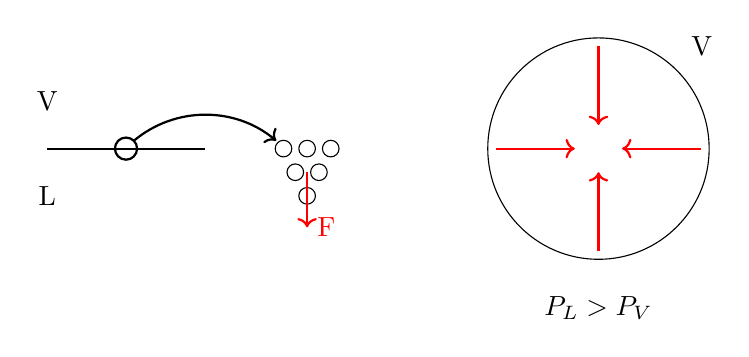
\begin{tikzpicture}
        \draw[thick] (-4,0) node[anchor=north,yshift=-10pt] {L} node[anchor=south,yshift=10pt] {V} -- (-2,0);
        \draw[thick] (-3,0) circle (4pt);
        \draw[thick,->] (-2.9,0.1) arc (130:50:40pt);
        \draw (-1,0) circle (3pt);
        \draw (-0.7,0) circle (3pt);
        \draw (-0.4,0) circle (3pt);
        \draw (-0.85,-0.3) circle (3pt);
        \draw (-0.55,-0.3) circle (3pt);
        \draw (-0.7,-0.6) circle (3pt);
        \draw[red,thick,->] (-0.7,-0.3) -- (-0.7,-1) node[anchor=west] {F};

        \draw (3,0) circle (40pt) node[anchor=south west,xshift=30pt,yshift=30pt] {V} node[anchor=north,yshift=-50pt] {$P_L > P_V$};
        \draw[thick,red,->] (3,1.3) -- (3,0.3);
        \draw[thick,red,->] (3,-1.3) -- (3,-0.3);
        \draw[thick,red,->] (1.7,0) -- (2.7,0);
        \draw[thick,red,->] (4.3,0) -- (3.3,0);
    \end{tikzpicture}
\end{figure}
The Young-Laplace equation relates the pressure difference $\Delta P$ between the two phases (e.g. water and air), and the geometry of the interface, assuming we can neglect gravity:
\begin{figure}[H]
    \centering
    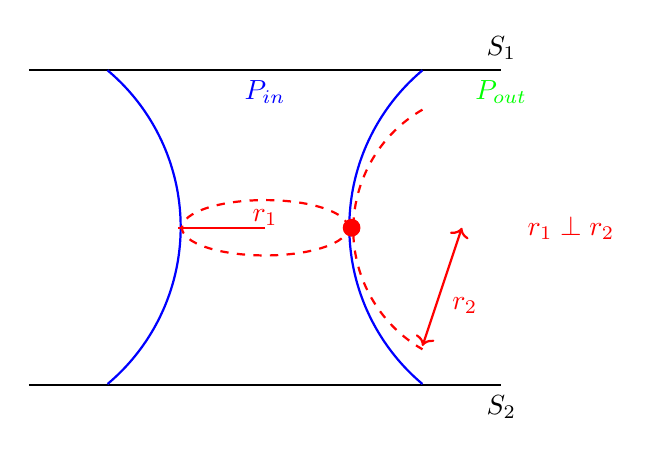
\begin{tikzpicture}
        \draw[thick] (-3,3) -- (3,3) node[anchor=south] {$S_1$} node[anchor=north,midway,blue] {$P_{in}$} node[anchor=north,green] {$P_{out}$};
        \draw[thick] (-3,-1) -- (3,-1) node[anchor=north] {$S_2$};
        \draw[thick,blue] (-2,3) arc (50:-50:74pt);
        \draw[thick,blue] (2,3) arc (130:230:74pt);
        \draw[red,dashed,thick] (0,1) ellipse (30pt and 10pt);
        \draw[red,thick] (0,1) node[anchor=south,yshift=-3pt] {$r_1$} -- (-1.1,1);
        \filldraw[red] (1.1,1) circle (3pt);
        \draw[thick,red,dashed] (2,2.5) arc (120:240:50pt);
        \draw[thick,<->,red] (2,-0.5) -- (2.5,1) node[anchor=north west,midway] {$r_2$} node[anchor=west,xshift=20pt] {$r_1 \perp r_2$};
    \end{tikzpicture}
\end{figure}
The Young-Laplace equation is as follows:
\begin{equation}
    \Delta P = P_{in} - P_{out} = \gamma_L \left(\frac{1}{r_1} + \frac{1}{r_2}\right)
\end{equation}
The Young-Laplace equation has several fundamental implications:
\begin{itemize}
    \item If we know the shape of a liquid surface, we can calculate the pressure difference across the surface.
    \item In the absence of external fields (e.g. gravity), the pressure is the same everywhere, otherwise the liquid would flow.
        This measn that the curvature needs to be the same everywhere across an interface at equilibrium.
    \item We can calculate the equilibrium shape of a liquid surface with the Laplace-Young equation.
        In practice, this is not trivial and often done using numerical methods on computers.
\end{itemize}
If the liquid structures considered are large enough, the influence of gravity (hydrostatic pressure) must also be taken into consideration.
The Young-Laplace equation becomes:
\begin{equation}
    \Delta P = \gamma_L \left(\frac{1}{r_1} + \frac{1}{r_2}\right) + \rho gh
\end{equation}
Practically, it is useful to define a capillary constant $\chi_c$ that has a length unit:
\begin{equation}
    \chi_c = \sqrt{\frac{\gamma_L}{\rho g}}, \text{ water - }\chi_c \approx 2.7nm
\end{equation}
For structures with radii of curvatures much smaller than $\chi_c$, the influence of gravity can be neglected.
The Young-Laplace equation is fundamental to modelling most capillary effects.
Hereafter we review a few of these effects.

\section{The Kelvin Equation}
The Young-Laplace equation links the geometry of a liquid surface (effectively intersface with another liquid or a vapour) to the difference in pressure $\Delta P$ through the interface at equilibrium.
The Young-Laplace equation is general in the sense that it simply relates curvature with a difference in pressure between inside and outside of the liquid, but does not specify the origin or implication of this pressure (gas pressure, vapour pressure).
In practice, it is often the vapour pressure, $P_0$, we care about: the pressure of a vapour phase at thermodynamic equilibrium with its liquid phase.
The vapour pressure effectively describes the ease with which a liquid will evaporate: a high vapour pressure indicates a strong tendency to evaporate while a low vapour pressure is associated with limited evaporation (i.e. few molecules in vapour phase).

It  is  important  to  realise  that  the  thermodynamic  definition  of $P_0$ assumes a \textit{flat interface} between the liquid and its vapour at equilibrium.
In the case of a curved droplet, we can still calculate a vapour pressure $P_V$, but it will not be equal to $P_0$ due to the interfacial effects described by the Young-Laplace equation.
The Kelvin equation describes how the vapour pressure is affected by the curvature of the liquid surface in contact with the vapour.
In other words, the Kelvin equation describes how liquid curvature changes the tendency for evaporation in a system.
To derive the Kelvin equation, we simply need to remember that at thermodynamic equilibrium, the chemical potential of the liquid molecules in the liquid meniscus and in the other medium (vapour, other liquid) must be equal.
In the case of a liquid at equilibrium with its vapour, for example a drop of water in air, we can use the ideal gas law to write the chemical potential explicitly:
\begin{align}
    V:~ \mu_V &= \mu_0 + k_BT\ln\left(\frac{P}{P_0}\right) \\
    L:~ \mu_L &= \mu_0 + V_m\,dP = \mu_0 + V_m\gamma_L\left(\frac{1}{r_1} + \frac{1}{r_2}\right)
\end{align}
where $V_m$ is the volume of one molecule.
By equating the two chemical potentuals, we obtain the Kelvin equation:
\begin{equation}
    k_BT\ln\left(\frac{P}{P_0}\right) = \gamma_LV_m\left(\frac{1}{r_1} + \frac{1}{r_2}\right)
\end{equation}
The Kelvin equation tells us that large liquid drops are more stable than smaller ones due to a lower relative vapour pressure.
The opposite is true for bubbles in a liquid since the sign of the curvature is inverted.

\section{Particles floating at the gas-liquid interface}
When placed at the surface of a liquid - a liquid-gas interface - small particles may get trapped, even if their density is higher than that of the liquid, provided their contact angle is not zero.
For simplicity, let's distinguish 'small' from 'large' particles:
\begin{itemize}
    \item We define as 'small' particles small enough so that gravity and buoyancy can be neglected in comparison with Brownian motion.
        Typically, small particles range up to $\approx 100\,\mu$m.
    \item By extension, large particles are defined as particles where the effect of gravity/buoyancy becomes appreciable.
\end{itemize}

\subsection{Large particles}
If gravity or buoyancy has the ability to move the particle perpendicularly to the interface, the surface of the liquid is deformed by the contact angle of the particle.
\begin{figure}[H]
    \centering
    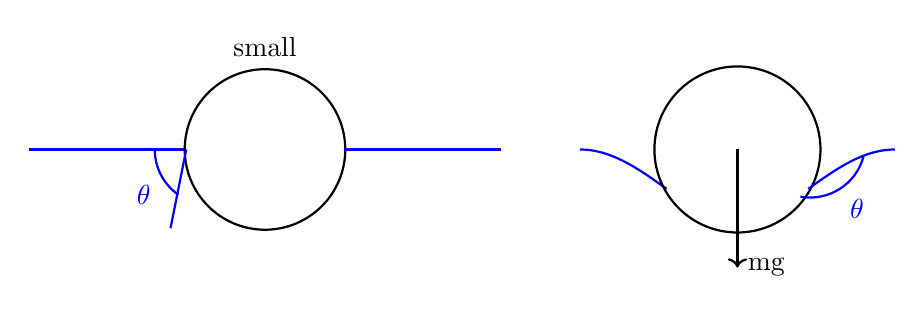
\begin{tikzpicture}
        \draw[thick,blue] (-3,0) -- (-1,0);
        \draw[thick] (0,0) circle (29pt) node[anchor=south,yshift=30pt] {small};
        \draw[blue,thick] (1,0) -- (3,0);
        \draw[blue,thick] (-1,0) -- (-1.2,-1);
        \draw[blue,thick] (-1.4,0) arc (180:235:20pt) node[anchor=north east,midway] {$\theta$};

        \draw[blue,thick] (4,0) cos (5.1,-0.5);
        \draw[thick] (6,0) circle (30pt);
        \draw[blue,thick] (6.9,-0.5) sin (8,0);
        \draw[blue,thick] (6.8,-0.6) arc (-100:-15:20pt) node[anchor=north west,midway] {$\theta$};
        \draw[thick,->] (6,0) -- (6,-1.5) node[anchor=west] {mg};
    \end{tikzpicture}
\end{figure}
Calculating the capillary force can be done if the curvature of the liquid around the particle is known.
Practically, this is done by equating the capillary pressure (from the Young-Laplace equation) to gravitational force, taking into account buoyancy.

\subsection{Small particles}
If the contact angle is zero (fully wetting), the particle sinks into the liquid where it diffuses through Brownian motion.
If the contact angle is larger than zero, the particle will position itself at the interface so that its contact angle can be satisfied without inducing any curvature of the liquid surface.
This makes calculations relatively straightforward.
Practically, to evaluate how stable is the particle when at the interface, it is useful to calculate the change in Gibbs $\Delta G$ free energy associated with removing the particle from this gas-liquid interface.
$\Delta G$ effectively quantifies the work needed to remove the particle  from  the  interface  and  hence  provides  important  information  in  many applications such as floatation (in mining) where we want the particles to remain at the interface.
We  calculate $\Delta G$ for the process of pushing the particle from its position at the interface to completely immersed inside the liquid. The area of the particle exposed to the gas phase is given by:
\begin{align}
    A &= \pi(r^2+h^2) = 2\pi R^2(1-\cos\theta) \\
    h &= R - R\cos\theta \\
    r &= R\sin\theta
\end{align}
When the particle is moved from the interface to the liquid, the particle-liquid interface increases by $A$ at the expense of the particle-gas interface, and the liquid-gas interfact increases by $\pi(R\sin\theta)^2$:
\begin{equation}
    \Delta G = \underbrace{2\pi R^2(1-\cos\theta)}_{A} (\gamma_{SL} - \gamma_{SV}) + \pi R^2\sin^2\theta \gamma_{LV}
\end{equation}
Using Young's equation, we can further simplify this to:
\begin{align}
    \gamma_{SL} - \gamma_{SV} &= -\gamma_{LV}\cos\theta \\
    \Delta G &= \pi R^2\gamma_L(\cos\theta - 1)^2
\end{align}

\chapter{}
\section{Outline}
\begin{itemize}
    \item Thermodynamics of liquid mixtures
        \begin{itemize}
            \item Entropy of mixing, $\Delta S_{mix}$
            \item Enthalpy of mixing, $\Delta H_{mix}$
            \item $\Delta G_{mix}$
        \end{itemize}
    \item $\Delta G_{mix}(\phi)$ - composition
    \item Regular solution model
\end{itemize}

Important concepts from last lecture
\begin{itemize}
    \item Wetting
        \begin{itemize}
            \item Young and Dupr\'{e}:
                \begin{equation}
                    W_{SL} = \gamma_L(1+\cos\theta)
                \end{equation}
        \end{itemize}
    \item Spreading (Young)
        \begin{equation}
            S_{ACB} = \gamma_{AB} - \gamma_{AC} - \gamma_{BC}
        \end{equation}
    \item Capillary effects
        \begin{itemize}
            \item Young-Laplace 
                \begin{equation}
                    \Delta P = \gamma_L\left(\frac{1}{r_1}+\frac{1}{r_2}\right)
                \end{equation}
            \item Kelvin
            \item Floating particle
        \end{itemize}
\end{itemize}

\section{Thermodynamics of liquid-liquid mixture}
We have seen previously that the Gibbs free energy $G$ is the natural thermodynamics potential for describing a system in ambient conditions (constant pressure and temperature).
At equilibrium, mixtures of liquids can also be described with $G$: for a given liquid, the difference $\Delta G$ between the liquid in a pure and mixed state quantifies the stability of the mixture. 
\begin{figure}[H]
    \centering
    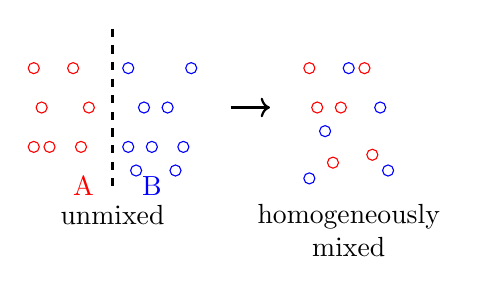
\begin{tikzpicture}
        \draw[thick,dashed] (0,2) -- (0,0) node[anchor=north,yshift=-3pt] {unmixed} node[anchor=east,red,xshift=-3pt] {A} node[anchor=west,blue,xshift=7pt] {B};

        \draw[red] (-1,1.5) circle (2pt);
        \draw[red] (-0.5,1.5) circle (2pt);
        \draw[red] (-0.3,1) circle (2pt);
        \draw[red] (-0.9,1) circle (2pt);
        \draw[red] (-0.8,0.5) circle (2pt);
        \draw[red] (-0.4,0.5) circle (2pt);
        \draw[red] (-1,0.5) circle (2pt);
            
        \draw[blue] (1,1.5) circle (2pt);
        \draw[blue] (0.2,1.5) circle (2pt);
        \draw[blue] (0.4,1) circle (2pt);
        \draw[blue] (0.7,1) circle (2pt);
        \draw[blue] (0.2,0.5) circle (2pt);
        \draw[blue] (0.5,0.5) circle (2pt);
        \draw[blue] (0.9,0.5) circle (2pt);
        \draw[blue] (0.3,0.2) circle (2pt);
        \draw[blue] (0.8,0.2) circle (2pt);

        \draw[thick,->] (1.5,1) -- (2,1);

        \draw[red] (2.5,1.5) circle (2pt);
        \draw[blue] (3,1.5) circle (2pt);
        \draw[red] (3.2,1.5) circle (2pt);
        \draw[red] (2.6,1) circle (2pt);
        \draw[red] (2.9,1) circle (2pt);
        \draw[blue] (3.4,1) circle (2pt);
        \draw[blue] (2.7,0.7) circle (2pt);
        \draw[red] (3.3,0.4) circle (2pt);
        \draw[blue] (2.5,0.1) circle (2pt);
        \draw[blue] (3.5,0.2) circle (2pt);
        \draw[red] (2.8,0.3) circle (2pt);
        \draw[white,dashed] (3,1) -- (3,-0.1) node[anchor=north,black,align=center] {homogeneously \\ mixed};
    \end{tikzpicture}
\end{figure}
Let's recall that:
\begin{align}
    \Delta G_{mix} &= G_{mix} - G_{unmixed} = \Delta H_{mix} - T\Delta S_{mix} \\
    \Delta G_{mix} &< 0 \text{ - spontaneous mixing} \\
    \Delta G_{mix} &> 0 \text{ - demix}
\end{align}
Let's consider a mixture of A in B characterised by the fraction $\phi_B$ of liquid A in the total mixture. 
If we ignore any mixing process, the average free energy per molecule in the system is simply the fraction-weighted average of the free energies of the pure liquid per molecule. 
\begin{figure}[H]
    \centering
    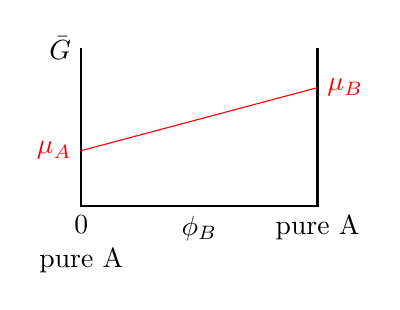
\begin{tikzpicture}
        \draw[thick] (0,2) node[anchor=east] {$\bar{G}$} -- (0,0) node[anchor=north,align=center] {0 \\ pure A} -- (3,0) node[anchor=north] {pure A} node[anchor=north,midway] {$\phi_B$} -- (3,2);
        \draw[red] (0,0.7) node[anchor=east] {$\mu_A$} -- (3,1.5) node[anchor=west] {$\mu_B$};
    \end{tikzpicture}
\end{figure}

\section{Change in entropy upon mixing}
When two liquids are mixed, the entropy always increases. 
$\Delta S > 0$ is the driving force for the mixing to proceed. 
The entropy of the mixture can be directly calculated from Boltzman's formula:
\begin{equation}
    \bar{S} = -k_B\sum_i\phi_i\ln(\phi_i)
\end{equation}
$\phi_i$ is the probability of finding molecule $i$ at a given location. 
For a binary mixture of liquids A and B, we only have two states: either a particular site is occupied by A or by B.
We can hence simplify the formula as follow:
\begin{align}
    \phi_A &= \frac{N_A}{N_A + N_B},~ \phi_B = \frac{N_B}{N_A+N_B},~ \phi_A + \phi_B = 1 \\
    \bar{S} &= -k_B\left[\phi_A\ln(\phi_A) + \phi_B\ln(\phi_B)\right]
\end{align}
\textbf{Note:} we could have derived the same formula from an explicit calculation for an ideal gas.
Let's assume we have the following system:
\begin{figure}[H]
    \centering
    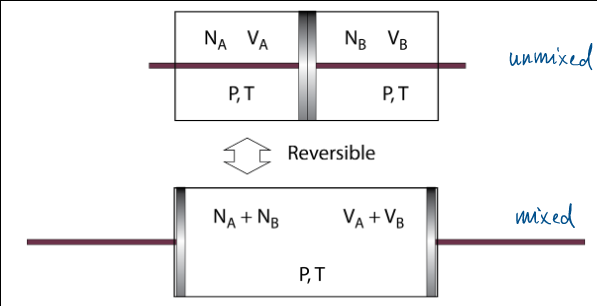
\includegraphics[scale=0.5]{piston.png}
\end{figure}
\begin{align} 
    PV &= Nk_BT,~ U \neq U(V) \\
    \Delta U &= 0 = W + q \implies W^{rev} = -Q^{rev}
\end{align}
From the first law of thermodynamics, we get:
\begin{align}
    W^{rev} &= \int_{V_A}^{V_A+V_B} -P_A\,dV + \int_{V_B}^{V_A+V_B} -P_V\,dV \\
            &= -\int_{V_A}^{V_A+V_B} \frac{N_Ak_BT}{V}\,dV - \int_{V_B}^{V_A+V_B}\frac{N_Bk_BT}{V}\,dV \\
            &= N_Ak_BT\ln\underbrace{\left(\frac{V_A}{V_A+V_B}\right)}_{\phi_A} + N_Bk_BT\ln\underbrace{\left(\frac{V_B}{V_B+V_A}\right)}_{\phi_B} = -Q^{rev} \\
    \Delta\bar{S}_{mix} &= \frac{Q^{rev}}{TN} = -\phi_Ak_B\ln(\phi_A) - \phi_Bk_B\ln(\phi_B) \geq 0 \\
    N &= N_A + N_B \\
    \phi_{A,B} &= \frac{N_{A,B}}{N} = \frac{V_{A,B}}{V_A+V_B}
\end{align}
This result can be generalised for more than two components, hence retrieving the Boltzmann formula.
Let's look at these results graphically:
\begin{figure}[H]
    \centering
    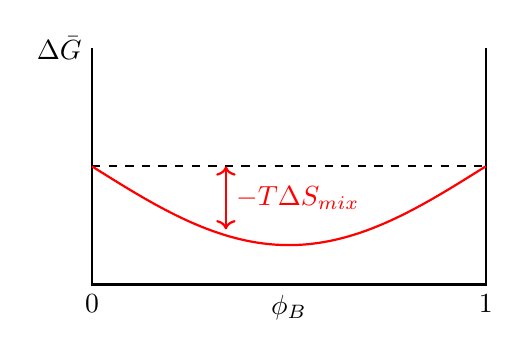
\begin{tikzpicture}
        \draw[thick] (0,3) node[anchor=east] {$\Delta\bar{G}$} -- (0,0) node[anchor=north] {0} -- (5,0) node[anchor=north] {1} node[anchor=north,midway] {$\phi_B$} -- (5,3);
        \draw[thick,dashed] (0,1.5) -- (5,1.5);
        \draw[red,thick] (0,1.5) sin (2.5,0.5) cos (5,1.5);
        \draw[red,thick,<->] (1.7,0.7) -- (1.7,1.5) node[anchor=west,midway] {$-T\Delta S_{mix}$};
    \end{tikzpicture}
\end{figure}

\section{Change in enthalpy upon mixing}
Ideal gases do not experience any change in enthalpy upon mixing due to the assumption that all species do not interact together. 
This is not true for most liquids and molecular interactions described by the enthalpy of the system. 
A simple expression can be derived from the different molecular interactions at play. 
Let's consider the case of a binary mixture of molecules of type A and B, with constant pressure and some molecular arrangement regardless of composition. 
\begin{align}
    \Delta\bar{U}_{mix} &= \bar{U}_{mix} - \bar{U}_{unmixed} \\
                        &= \begin{pmatrix} \text{energy change} \\ \text{per A-B bond} \\ \text{relative to A-A} \\ \text{or B-B} \end{pmatrix} (\text{\# A-B contacts}) \\
    P_{A-B} &\approx \phi_A\phi_Bz \\
    \Delta\bar{U}_{mix} &= \chi\phi_A\phi_B \\
    H &\equiv U + PV \\
    \Delta\bar{H}_{mix} &= \Delta\bar{U}_{mix} + P\cancel{\Delta V_{mix}} + V\cancel{\Delta P_{mix}} \\
    \Delta\bar{H}_{mix} &= \chi\phi_A\phi_B
\end{align}
Let's look at the enthalpy of mixing graphically:
\begin{figure}[H]
    \centering
    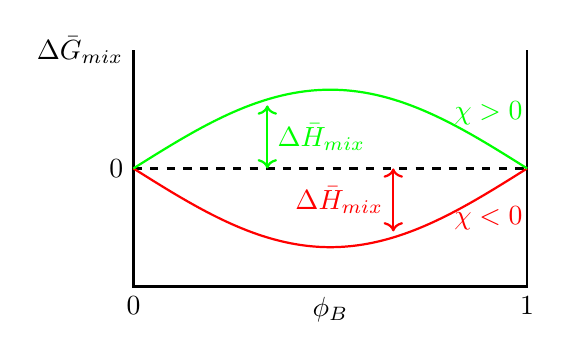
\begin{tikzpicture}
        \draw[thick] (0,3) node[anchor=east] {$\Delta\bar{G}_{mix}$} -- (0,0) node[anchor=north] {0} -- (5,0) node[anchor=north] {1} node[anchor=north,midway] {$\phi_B$} -- (5,3);
        \draw[thick,dashed] (0,1.5) node[anchor=east] {0} -- (5,1.5);
        \draw[red,thick] (0,1.5) sin (2.5,0.5) cos (5,1.5) node[anchor=north,xshift=-14pt,yshift=-10pt] {$\chi < 0$};
        \draw[red,thick,<->] (3.3,0.7) -- (3.3,1.5) node[anchor=east,midway] {$\Delta \bar{H}_{mix}$};

        \draw[green,thick] (0,1.5) sin (2.5,2.5) cos (5,1.5) node[anchor=south,xshift=-14pt,yshift=12pt] {$\chi > 0$};
        \draw[green,thick,<->] (1.7,2.3) -- (1.7,1.5) node[anchor=west,midway] {$\Delta \bar{H}_{mix}$};
    \end{tikzpicture}
\end{figure}
We can combine the expression found for enthalpy and entropy and derive \textbf{the change in Gibbs free energy upon mixing.}
\begin{align}
    \Delta\bar{G}_{mix}^{RS} &= \Delta\bar{H}_{mix} - T\Delta\bar{S}_{mix} \\
                             &= \chi\phi_A\phi_B + k_BT\underbrace{\left[\phi_A\ln(\phi_A) + \phi_B\ln(\phi_B)\right]}_{\leq 0} 
\end{align}
This is the \textbf{regular solution model.}
\begin{itemize}
    \item $\phi_A+\phi_B=1$
    \item $x > 0$ disfavours mixing
    \item $x > 0$ favours mixing
\end{itemize}
Let's look at the changes in mixing entropy and enthalpy graphically:
\begin{figure}[H]
    \centering
    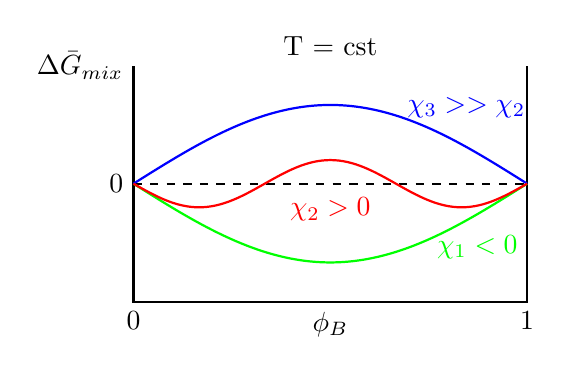
\begin{tikzpicture}
        \draw[thick] (0,3) node[anchor=east] {$\Delta\bar{G}_{mix}$} -- (0,0) node[anchor=north] {0} -- (5,0) node[anchor=north] {1} node[anchor=north,midway] {$\phi_B$} -- (5,3);
        \draw[thick,dashed] (0,1.5) node[anchor=east] {0} -- (5,1.5);
        \draw[white] (0,3) -- (5,3) node[anchor=south,midway,black] {T = cst};
        \draw[green,thick] (0,1.5) sin (2.5,0.5) cos (5,1.5) node[anchor=north,xshift=-18pt,yshift=-15pt] {$\chi_1 < 0$};
        \draw[blue,thick] (0,1.5) sin (2.5,2.5) cos (5,1.5) node[anchor=south,xshift=-22pt,yshift=20pt] {$\chi_3 >> \chi_2$};
        \draw[red,thick] (0,1.5) sin (5/6,1.2) cos (5/3,1.5) sin (2.5,1.8) node[anchor=north,yshift=-10pt] {$\chi_2 > 0$} cos (10/3,1.5) sin (25/6,1.2) cos (5,1.5);
    \end{tikzpicture}
    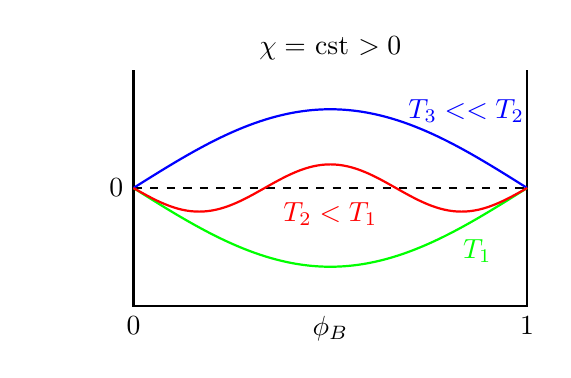
\begin{tikzpicture}
        \draw[thick] (0,3) node[white,anchor=east] {$\Delta\bar{G}_{mix}$} -- (0,0) node[anchor=north] {0} -- (5,0) node[anchor=north] {1} node[anchor=north,midway] {$\phi_B$} -- (5,3);
        \draw[thick,dashed] (0,1.5) node[anchor=east] {0} -- (5,1.5);
        \draw[white] (0,3) -- (5,3) node[anchor=south,midway,black] {$\chi =$ cst $> 0$};
        \draw[green,thick] (0,1.5) sin (2.5,0.5) cos (5,1.5) node[anchor=north,xshift=-18pt,yshift=-15pt] {$T_1$};
        \draw[blue,thick] (0,1.5) sin (2.5,2.5) cos (5,1.5) node[anchor=south,xshift=-22pt,yshift=20pt] {$T_3 << T_2$};
        \draw[red,thick] (0,1.5) sin (5/6,1.2) cos (5/3,1.5) sin (2.5,1.8) node[anchor=north,yshift=-10pt] {$T_2 < T_1$} cos (10/3,1.5) sin (25/6,1.2) cos (5,1.5);
    \end{tikzpicture}
\end{figure}

\chapter{}
\section{Outline}
\begin{itemize}
    \item Predictions from the Regular Solution Model
        \begin{itemize}
            \item Fate of mixture
            \item Stability of mixture
            \item Phase diageam
        \end{itemize}
    \item Molecular view of mixing/demixing
\end{itemize}

Important concepts from last lecture:
\begin{align}
    \Delta\bar{G}_{mix} &= \bar{G}_{mix} - \bar{G}_{unmixed} \\
                        &= \underbrace{\Delta\bar{H}_{mix}}_{\chi\phi_A\phi_B} - T\times\underbrace{\Delta\bar{S}_{mix}}_{-k_B[\phi_A\ln\phi_A+\phi_B\ln\phi_B]}
\end{align}
$\phi_{A,B}$ - molecular fraction of A,B
\begin{align}
    \Delta\bar{G}_{mix} &\begin{cases} > 0 \\ < 0 \\ = 0\end{cases} \\
    \Delta\bar{G}_{mix}^{RS} &= \chi\phi(1-\phi) + k_BT[\phi\ln\phi + (1-\phi)\ln(1-\phi)] \\
    \phi &= \phi_B,~ \phi_A = 1 - \phi
\end{align}
\begin{figure}[H]
    \centering
    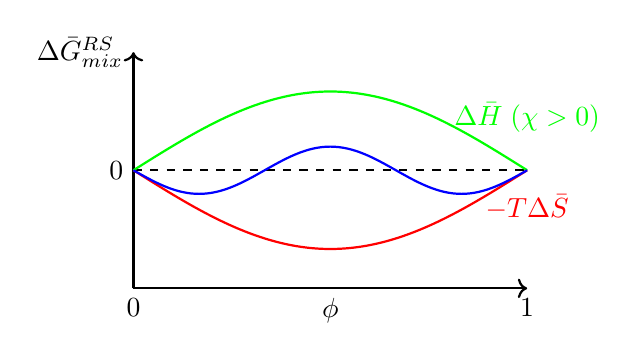
\begin{tikzpicture}
        \draw[thick,->] (0,0) -- (0,3) node[anchor=east,midway] {0} node[anchor=east] {$\Delta\bar{G}_{mix}^{RS}$};
        \draw[thick,->] (0,0) node[anchor=north] {0} -- (5,0) node[anchor=north] {1} node[anchor=north,midway] {$\phi$};
        \draw[dashed,thick] (0,1.5) -- (5,1.5);
        \draw[red,thick] (0,1.5) sin (2.5,0.5) cos (5,1.5) node[anchor=north,yshift=-5pt] {$-T\Delta\bar{S}$};
        \draw[green,thick] (0,1.5) sin (2.5,2.5) cos (5,1.5) node[anchor=south,yshift=10pt] {$\Delta\bar{H}\; (\chi > 0)$};
        \draw[blue,thick] (0,1.5) sin (5/6,1.2) cos (5/3,1.5) sin (2.5,1.8) cos (10/3,1.5) sin (25/6,1.2) cos (5,1.5);
    \end{tikzpicture}
\end{figure}

\section{The Regular Solution Model: A molecular level perspective}
\begin{multicols}{2}
    Let's look at an unmixed solution: 
    \begin{figure}[H]
        \centering
        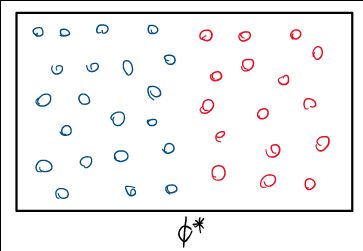
\includegraphics[scale=0.5]{unmix.png}
    \end{figure}
    \columnbreak
    The total free energy is:
    \begin{figure}[H]
        \centering
        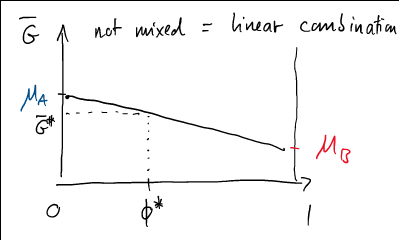
\includegraphics[scale=0.5]{unmixfree.png}
    \end{figure}
\end{multicols}
\begin{multicols}{2}
    When we mix it homogeneously:
    \begin{figure}[H]
        \centering
        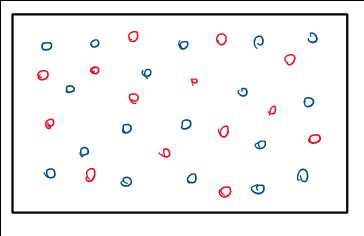
\includegraphics[scale=0.5]{homo.png}
    \end{figure}
    \columnbreak
    The change in free energy (from unmixed solution) is:
    \begin{figure}[H]
        \centering
        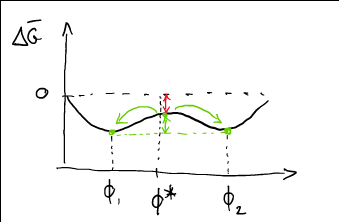
\includegraphics[scale=0.5]{homofree.png}
    \end{figure}
\end{multicols}
Why do we have local minima in free energy and what do they represent in terms of molecular organisation?
\begin{figure}[H]
    \centering
    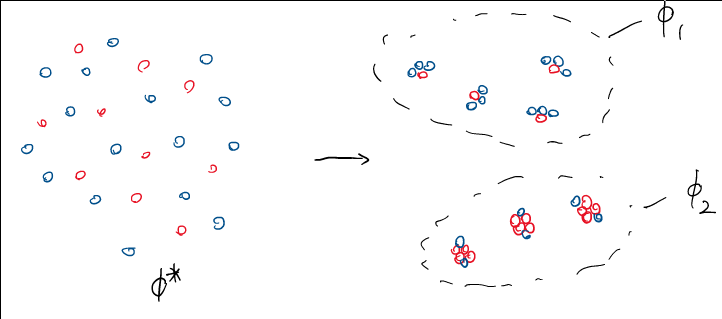
\includegraphics[scale=0.5]{locals.png}
\end{figure}

\section{From the Regular Solution Model to phase diagrams}
The change in Gibbs free energy is
\begin{equation}
    \Delta\bar{G}_{mix}^{rs} = \chi\phi_A\phi_B + kT(\phi_A\ln\phi_a + \phi_B\ln\phi_B)
\end{equation}
This model is known as the \textbf{regular solution model.}
Let's look at the behaviour of regular solutions graphically:
\begin{equation}
    \bar{G}_{mix} = \bar{G}_{unmix} + \Delta\bar{G}_{mix}
\end{equation}
\begin{figure}[H]
    \centering
    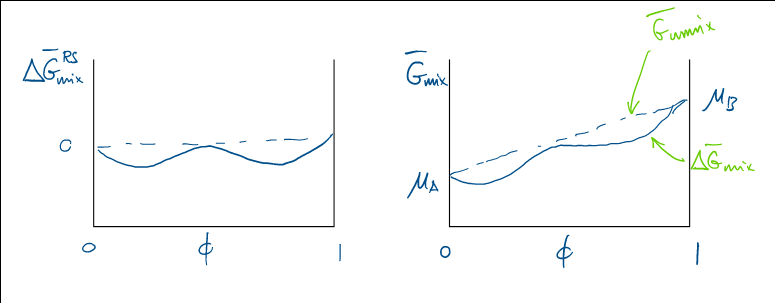
\includegraphics[scale=0.5]{behave.png}
\end{figure}
The free energy of mixing of the system varies with both $\chi$ and temperature:
\begin{figure}[H]
    \centering
    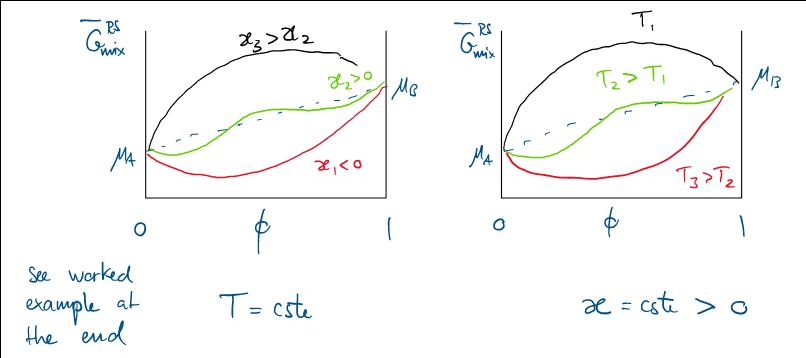
\includegraphics[scale=0.5]{behive.png}
\end{figure}
page 4

























\end{document}
